% Created by tikzDevice version 0.9 on 2016-03-14 23:41:49
% !TEX encoding = UTF-8 Unicode
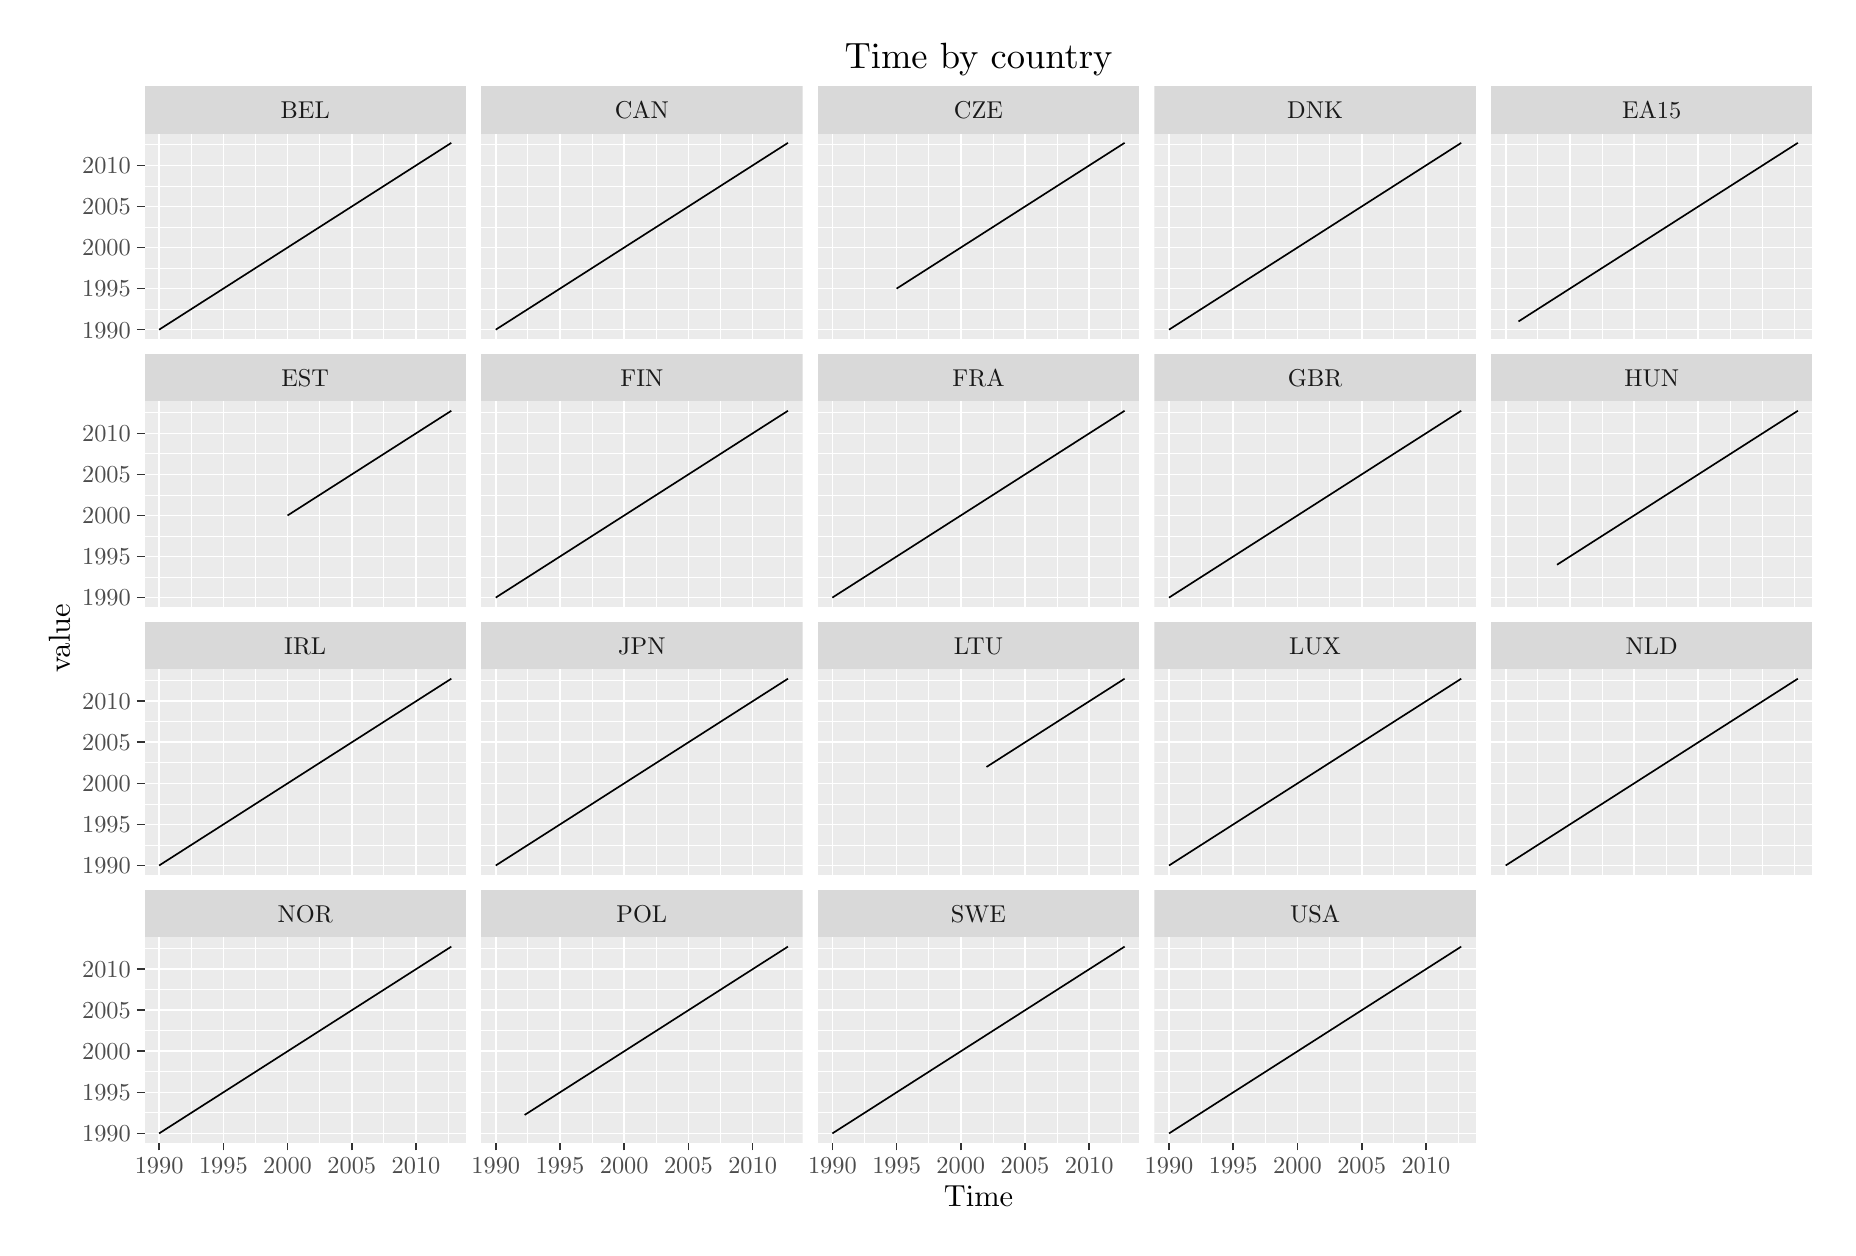
\begin{tikzpicture}[x=1pt,y=1pt]
\definecolor{fillColor}{RGB}{255,255,255}
\path[use as bounding box,fill=fillColor,fill opacity=0.00] (0,0) rectangle (650.43,433.62);
\begin{scope}
\path[clip] (  0.00,  0.00) rectangle (650.43,433.62);
\definecolor{drawColor}{RGB}{255,255,255}
\definecolor{fillColor}{RGB}{255,255,255}

\path[draw=drawColor,line width= 0.6pt,line join=round,line cap=round,fill=fillColor] (  0.00,  0.00) rectangle (650.43,433.62);
\end{scope}
\begin{scope}
\path[clip] ( 42.22,321.12) rectangle (158.36,395.37);
\definecolor{fillColor}{gray}{0.92}

\path[fill=fillColor] ( 42.22,321.12) rectangle (158.36,395.37);
\definecolor{drawColor}{RGB}{255,255,255}

\path[draw=drawColor,line width= 0.3pt,line join=round] ( 42.22,331.91) --
	(158.36,331.91);

\path[draw=drawColor,line width= 0.3pt,line join=round] ( 42.22,346.75) --
	(158.36,346.75);

\path[draw=drawColor,line width= 0.3pt,line join=round] ( 42.22,361.58) --
	(158.36,361.58);

\path[draw=drawColor,line width= 0.3pt,line join=round] ( 42.22,376.42) --
	(158.36,376.42);

\path[draw=drawColor,line width= 0.3pt,line join=round] ( 42.22,391.25) --
	(158.36,391.25);

\path[draw=drawColor,line width= 0.3pt,line join=round] ( 59.10,321.12) --
	( 59.10,395.37);

\path[draw=drawColor,line width= 0.3pt,line join=round] ( 82.31,321.12) --
	( 82.31,395.37);

\path[draw=drawColor,line width= 0.3pt,line join=round] (105.51,321.12) --
	(105.51,395.37);

\path[draw=drawColor,line width= 0.3pt,line join=round] (128.72,321.12) --
	(128.72,395.37);

\path[draw=drawColor,line width= 0.3pt,line join=round] (151.92,321.12) --
	(151.92,395.37);

\path[draw=drawColor,line width= 0.6pt,line join=round] ( 42.22,324.49) --
	(158.36,324.49);

\path[draw=drawColor,line width= 0.6pt,line join=round] ( 42.22,339.33) --
	(158.36,339.33);

\path[draw=drawColor,line width= 0.6pt,line join=round] ( 42.22,354.16) --
	(158.36,354.16);

\path[draw=drawColor,line width= 0.6pt,line join=round] ( 42.22,369.00) --
	(158.36,369.00);

\path[draw=drawColor,line width= 0.6pt,line join=round] ( 42.22,383.83) --
	(158.36,383.83);

\path[draw=drawColor,line width= 0.6pt,line join=round] ( 47.50,321.12) --
	( 47.50,395.37);

\path[draw=drawColor,line width= 0.6pt,line join=round] ( 70.71,321.12) --
	( 70.71,395.37);

\path[draw=drawColor,line width= 0.6pt,line join=round] ( 93.91,321.12) --
	( 93.91,395.37);

\path[draw=drawColor,line width= 0.6pt,line join=round] (117.12,321.12) --
	(117.12,395.37);

\path[draw=drawColor,line width= 0.6pt,line join=round] (140.32,321.12) --
	(140.32,395.37);
\definecolor{drawColor}{RGB}{0,0,0}

\path[draw=drawColor,line width= 0.6pt,line join=round] ( 47.50,324.49) --
	( 48.66,325.24) --
	( 49.82,325.98) --
	( 50.98,326.72) --
	( 52.14,327.46) --
	( 53.30,328.20) --
	( 54.46,328.94) --
	( 55.62,329.69) --
	( 56.78,330.43) --
	( 57.94,331.17) --
	( 59.10,331.91) --
	( 60.26,332.65) --
	( 61.42,333.39) --
	( 62.58,334.14) --
	( 63.74,334.88) --
	( 64.90,335.62) --
	( 66.07,336.36) --
	( 67.23,337.10) --
	( 68.39,337.84) --
	( 69.55,338.59) --
	( 70.71,339.33) --
	( 71.87,340.07) --
	( 73.03,340.81) --
	( 74.19,341.55) --
	( 75.35,342.30) --
	( 76.51,343.04) --
	( 77.67,343.78) --
	( 78.83,344.52) --
	( 79.99,345.26) --
	( 81.15,346.00) --
	( 82.31,346.75) --
	( 83.47,347.49) --
	( 84.63,348.23) --
	( 85.79,348.97) --
	( 86.95,349.71) --
	( 88.11,350.45) --
	( 89.27,351.20) --
	( 90.43,351.94) --
	( 91.59,352.68) --
	( 92.75,353.42) --
	( 93.91,354.16) --
	( 95.07,354.91) --
	( 96.23,355.65) --
	( 97.39,356.39) --
	( 98.55,357.13) --
	( 99.71,357.87) --
	(100.87,358.61) --
	(102.03,359.36) --
	(103.19,360.10) --
	(104.35,360.84) --
	(105.51,361.58) --
	(106.67,362.32) --
	(107.83,363.06) --
	(108.99,363.81) --
	(110.15,364.55) --
	(111.32,365.29) --
	(112.48,366.03) --
	(113.64,366.77) --
	(114.80,367.52) --
	(115.96,368.26) --
	(117.12,369.00) --
	(118.28,369.74) --
	(119.44,370.48) --
	(120.60,371.22) --
	(121.76,371.97) --
	(122.92,372.71) --
	(124.08,373.45) --
	(125.24,374.19) --
	(126.40,374.93) --
	(127.56,375.67) --
	(128.72,376.42) --
	(129.88,377.16) --
	(131.04,377.90) --
	(132.20,378.64) --
	(133.36,379.38) --
	(134.52,380.12) --
	(135.68,380.87) --
	(136.84,381.61) --
	(138.00,382.35) --
	(139.16,383.09) --
	(140.32,383.83) --
	(141.48,384.58) --
	(142.64,385.32) --
	(143.80,386.06) --
	(144.96,386.80) --
	(146.12,387.54) --
	(147.28,388.28) --
	(148.44,389.03) --
	(149.60,389.77) --
	(150.76,390.51) --
	(151.92,391.25) --
	(153.08,391.99);
\end{scope}
\begin{scope}
\path[clip] (163.86,321.12) rectangle (280.01,395.37);
\definecolor{fillColor}{gray}{0.92}

\path[fill=fillColor] (163.86,321.12) rectangle (280.01,395.37);
\definecolor{drawColor}{RGB}{255,255,255}

\path[draw=drawColor,line width= 0.3pt,line join=round] (163.86,331.91) --
	(280.01,331.91);

\path[draw=drawColor,line width= 0.3pt,line join=round] (163.86,346.75) --
	(280.01,346.75);

\path[draw=drawColor,line width= 0.3pt,line join=round] (163.86,361.58) --
	(280.01,361.58);

\path[draw=drawColor,line width= 0.3pt,line join=round] (163.86,376.42) --
	(280.01,376.42);

\path[draw=drawColor,line width= 0.3pt,line join=round] (163.86,391.25) --
	(280.01,391.25);

\path[draw=drawColor,line width= 0.3pt,line join=round] (180.75,321.12) --
	(180.75,395.37);

\path[draw=drawColor,line width= 0.3pt,line join=round] (203.95,321.12) --
	(203.95,395.37);

\path[draw=drawColor,line width= 0.3pt,line join=round] (227.16,321.12) --
	(227.16,395.37);

\path[draw=drawColor,line width= 0.3pt,line join=round] (250.36,321.12) --
	(250.36,395.37);

\path[draw=drawColor,line width= 0.3pt,line join=round] (273.57,321.12) --
	(273.57,395.37);

\path[draw=drawColor,line width= 0.6pt,line join=round] (163.86,324.49) --
	(280.01,324.49);

\path[draw=drawColor,line width= 0.6pt,line join=round] (163.86,339.33) --
	(280.01,339.33);

\path[draw=drawColor,line width= 0.6pt,line join=round] (163.86,354.16) --
	(280.01,354.16);

\path[draw=drawColor,line width= 0.6pt,line join=round] (163.86,369.00) --
	(280.01,369.00);

\path[draw=drawColor,line width= 0.6pt,line join=round] (163.86,383.83) --
	(280.01,383.83);

\path[draw=drawColor,line width= 0.6pt,line join=round] (169.14,321.12) --
	(169.14,395.37);

\path[draw=drawColor,line width= 0.6pt,line join=round] (192.35,321.12) --
	(192.35,395.37);

\path[draw=drawColor,line width= 0.6pt,line join=round] (215.55,321.12) --
	(215.55,395.37);

\path[draw=drawColor,line width= 0.6pt,line join=round] (238.76,321.12) --
	(238.76,395.37);

\path[draw=drawColor,line width= 0.6pt,line join=round] (261.96,321.12) --
	(261.96,395.37);
\definecolor{drawColor}{RGB}{0,0,0}

\path[draw=drawColor,line width= 0.6pt,line join=round] (169.14,324.49) --
	(170.30,325.24) --
	(171.46,325.98) --
	(172.62,326.72) --
	(173.78,327.46) --
	(174.94,328.20) --
	(176.10,328.94) --
	(177.26,329.69) --
	(178.42,330.43) --
	(179.58,331.17) --
	(180.75,331.91) --
	(181.91,332.65) --
	(183.07,333.39) --
	(184.23,334.14) --
	(185.39,334.88) --
	(186.55,335.62) --
	(187.71,336.36) --
	(188.87,337.10) --
	(190.03,337.84) --
	(191.19,338.59) --
	(192.35,339.33) --
	(193.51,340.07) --
	(194.67,340.81) --
	(195.83,341.55) --
	(196.99,342.30) --
	(198.15,343.04) --
	(199.31,343.78) --
	(200.47,344.52) --
	(201.63,345.26) --
	(202.79,346.00) --
	(203.95,346.75) --
	(205.11,347.49) --
	(206.27,348.23) --
	(207.43,348.97) --
	(208.59,349.71) --
	(209.75,350.45) --
	(210.91,351.20) --
	(212.07,351.94) --
	(213.23,352.68) --
	(214.39,353.42) --
	(215.55,354.16) --
	(216.71,354.91) --
	(217.87,355.65) --
	(219.03,356.39) --
	(220.19,357.13) --
	(221.35,357.87) --
	(222.51,358.61) --
	(223.67,359.36) --
	(224.83,360.10) --
	(226.00,360.84) --
	(227.16,361.58) --
	(228.32,362.32) --
	(229.48,363.06) --
	(230.64,363.81) --
	(231.80,364.55) --
	(232.96,365.29) --
	(234.12,366.03) --
	(235.28,366.77) --
	(236.44,367.52) --
	(237.60,368.26) --
	(238.76,369.00) --
	(239.92,369.74) --
	(241.08,370.48) --
	(242.24,371.22) --
	(243.40,371.97) --
	(244.56,372.71) --
	(245.72,373.45) --
	(246.88,374.19) --
	(248.04,374.93) --
	(249.20,375.67) --
	(250.36,376.42) --
	(251.52,377.16) --
	(252.68,377.90) --
	(253.84,378.64) --
	(255.00,379.38) --
	(256.16,380.12) --
	(257.32,380.87) --
	(258.48,381.61) --
	(259.64,382.35) --
	(260.80,383.09) --
	(261.96,383.83) --
	(263.12,384.58) --
	(264.28,385.32) --
	(265.44,386.06) --
	(266.60,386.80) --
	(267.76,387.54) --
	(268.92,388.28) --
	(270.08,389.03) --
	(271.25,389.77) --
	(272.41,390.51) --
	(273.57,391.25) --
	(274.73,391.99);
\end{scope}
\begin{scope}
\path[clip] (285.51,321.12) rectangle (401.65,395.37);
\definecolor{fillColor}{gray}{0.92}

\path[fill=fillColor] (285.51,321.12) rectangle (401.65,395.37);
\definecolor{drawColor}{RGB}{255,255,255}

\path[draw=drawColor,line width= 0.3pt,line join=round] (285.51,331.91) --
	(401.65,331.91);

\path[draw=drawColor,line width= 0.3pt,line join=round] (285.51,346.75) --
	(401.65,346.75);

\path[draw=drawColor,line width= 0.3pt,line join=round] (285.51,361.58) --
	(401.65,361.58);

\path[draw=drawColor,line width= 0.3pt,line join=round] (285.51,376.42) --
	(401.65,376.42);

\path[draw=drawColor,line width= 0.3pt,line join=round] (285.51,391.25) --
	(401.65,391.25);

\path[draw=drawColor,line width= 0.3pt,line join=round] (302.39,321.12) --
	(302.39,395.37);

\path[draw=drawColor,line width= 0.3pt,line join=round] (325.59,321.12) --
	(325.59,395.37);

\path[draw=drawColor,line width= 0.3pt,line join=round] (348.80,321.12) --
	(348.80,395.37);

\path[draw=drawColor,line width= 0.3pt,line join=round] (372.00,321.12) --
	(372.00,395.37);

\path[draw=drawColor,line width= 0.3pt,line join=round] (395.21,321.12) --
	(395.21,395.37);

\path[draw=drawColor,line width= 0.6pt,line join=round] (285.51,324.49) --
	(401.65,324.49);

\path[draw=drawColor,line width= 0.6pt,line join=round] (285.51,339.33) --
	(401.65,339.33);

\path[draw=drawColor,line width= 0.6pt,line join=round] (285.51,354.16) --
	(401.65,354.16);

\path[draw=drawColor,line width= 0.6pt,line join=round] (285.51,369.00) --
	(401.65,369.00);

\path[draw=drawColor,line width= 0.6pt,line join=round] (285.51,383.83) --
	(401.65,383.83);

\path[draw=drawColor,line width= 0.6pt,line join=round] (290.78,321.12) --
	(290.78,395.37);

\path[draw=drawColor,line width= 0.6pt,line join=round] (313.99,321.12) --
	(313.99,395.37);

\path[draw=drawColor,line width= 0.6pt,line join=round] (337.19,321.12) --
	(337.19,395.37);

\path[draw=drawColor,line width= 0.6pt,line join=round] (360.40,321.12) --
	(360.40,395.37);

\path[draw=drawColor,line width= 0.6pt,line join=round] (383.60,321.12) --
	(383.60,395.37);
\definecolor{drawColor}{RGB}{0,0,0}

\path[draw=drawColor,line width= 0.6pt,line join=round] (313.99,339.33) --
	(315.15,340.07) --
	(316.31,340.81) --
	(317.47,341.55) --
	(318.63,342.30) --
	(319.79,343.04) --
	(320.95,343.78) --
	(322.11,344.52) --
	(323.27,345.26) --
	(324.43,346.00) --
	(325.59,346.75) --
	(326.75,347.49) --
	(327.91,348.23) --
	(329.07,348.97) --
	(330.23,349.71) --
	(331.39,350.45) --
	(332.55,351.20) --
	(333.71,351.94) --
	(334.87,352.68) --
	(336.03,353.42) --
	(337.19,354.16) --
	(338.35,354.91) --
	(339.51,355.65) --
	(340.68,356.39) --
	(341.84,357.13) --
	(343.00,357.87) --
	(344.16,358.61) --
	(345.32,359.36) --
	(346.48,360.10) --
	(347.64,360.84) --
	(348.80,361.58) --
	(349.96,362.32) --
	(351.12,363.06) --
	(352.28,363.81) --
	(353.44,364.55) --
	(354.60,365.29) --
	(355.76,366.03) --
	(356.92,366.77) --
	(358.08,367.52) --
	(359.24,368.26) --
	(360.40,369.00) --
	(361.56,369.74) --
	(362.72,370.48) --
	(363.88,371.22) --
	(365.04,371.97) --
	(366.20,372.71) --
	(367.36,373.45) --
	(368.52,374.19) --
	(369.68,374.93) --
	(370.84,375.67) --
	(372.00,376.42) --
	(373.16,377.16) --
	(374.32,377.90) --
	(375.48,378.64) --
	(376.64,379.38) --
	(377.80,380.12) --
	(378.96,380.87) --
	(380.12,381.61) --
	(381.28,382.35) --
	(382.44,383.09) --
	(383.60,383.83) --
	(384.76,384.58) --
	(385.93,385.32) --
	(387.09,386.06) --
	(388.25,386.80) --
	(389.41,387.54) --
	(390.57,388.28) --
	(391.73,389.03) --
	(392.89,389.77) --
	(394.05,390.51) --
	(395.21,391.25) --
	(396.37,391.99);
\end{scope}
\begin{scope}
\path[clip] (407.15,321.12) rectangle (523.29,395.37);
\definecolor{fillColor}{gray}{0.92}

\path[fill=fillColor] (407.15,321.12) rectangle (523.29,395.37);
\definecolor{drawColor}{RGB}{255,255,255}

\path[draw=drawColor,line width= 0.3pt,line join=round] (407.15,331.91) --
	(523.29,331.91);

\path[draw=drawColor,line width= 0.3pt,line join=round] (407.15,346.75) --
	(523.29,346.75);

\path[draw=drawColor,line width= 0.3pt,line join=round] (407.15,361.58) --
	(523.29,361.58);

\path[draw=drawColor,line width= 0.3pt,line join=round] (407.15,376.42) --
	(523.29,376.42);

\path[draw=drawColor,line width= 0.3pt,line join=round] (407.15,391.25) --
	(523.29,391.25);

\path[draw=drawColor,line width= 0.3pt,line join=round] (424.03,321.12) --
	(424.03,395.37);

\path[draw=drawColor,line width= 0.3pt,line join=round] (447.23,321.12) --
	(447.23,395.37);

\path[draw=drawColor,line width= 0.3pt,line join=round] (470.44,321.12) --
	(470.44,395.37);

\path[draw=drawColor,line width= 0.3pt,line join=round] (493.64,321.12) --
	(493.64,395.37);

\path[draw=drawColor,line width= 0.3pt,line join=round] (516.85,321.12) --
	(516.85,395.37);

\path[draw=drawColor,line width= 0.6pt,line join=round] (407.15,324.49) --
	(523.29,324.49);

\path[draw=drawColor,line width= 0.6pt,line join=round] (407.15,339.33) --
	(523.29,339.33);

\path[draw=drawColor,line width= 0.6pt,line join=round] (407.15,354.16) --
	(523.29,354.16);

\path[draw=drawColor,line width= 0.6pt,line join=round] (407.15,369.00) --
	(523.29,369.00);

\path[draw=drawColor,line width= 0.6pt,line join=round] (407.15,383.83) --
	(523.29,383.83);

\path[draw=drawColor,line width= 0.6pt,line join=round] (412.43,321.12) --
	(412.43,395.37);

\path[draw=drawColor,line width= 0.6pt,line join=round] (435.63,321.12) --
	(435.63,395.37);

\path[draw=drawColor,line width= 0.6pt,line join=round] (458.84,321.12) --
	(458.84,395.37);

\path[draw=drawColor,line width= 0.6pt,line join=round] (482.04,321.12) --
	(482.04,395.37);

\path[draw=drawColor,line width= 0.6pt,line join=round] (505.25,321.12) --
	(505.25,395.37);
\definecolor{drawColor}{RGB}{0,0,0}

\path[draw=drawColor,line width= 0.6pt,line join=round] (412.43,324.49) --
	(413.59,325.24) --
	(414.75,325.98) --
	(415.91,326.72) --
	(417.07,327.46) --
	(418.23,328.20) --
	(419.39,328.94) --
	(420.55,329.69) --
	(421.71,330.43) --
	(422.87,331.17) --
	(424.03,331.91) --
	(425.19,332.65) --
	(426.35,333.39) --
	(427.51,334.14) --
	(428.67,334.88) --
	(429.83,335.62) --
	(430.99,336.36) --
	(432.15,337.10) --
	(433.31,337.84) --
	(434.47,338.59) --
	(435.63,339.33) --
	(436.79,340.07) --
	(437.95,340.81) --
	(439.11,341.55) --
	(440.27,342.30) --
	(441.43,343.04) --
	(442.59,343.78) --
	(443.75,344.52) --
	(444.91,345.26) --
	(446.07,346.00) --
	(447.23,346.75) --
	(448.39,347.49) --
	(449.55,348.23) --
	(450.71,348.97) --
	(451.87,349.71) --
	(453.03,350.45) --
	(454.20,351.20) --
	(455.36,351.94) --
	(456.52,352.68) --
	(457.68,353.42) --
	(458.84,354.16) --
	(460.00,354.91) --
	(461.16,355.65) --
	(462.32,356.39) --
	(463.48,357.13) --
	(464.64,357.87) --
	(465.80,358.61) --
	(466.96,359.36) --
	(468.12,360.10) --
	(469.28,360.84) --
	(470.44,361.58) --
	(471.60,362.32) --
	(472.76,363.06) --
	(473.92,363.81) --
	(475.08,364.55) --
	(476.24,365.29) --
	(477.40,366.03) --
	(478.56,366.77) --
	(479.72,367.52) --
	(480.88,368.26) --
	(482.04,369.00) --
	(483.20,369.74) --
	(484.36,370.48) --
	(485.52,371.22) --
	(486.68,371.97) --
	(487.84,372.71) --
	(489.00,373.45) --
	(490.16,374.19) --
	(491.32,374.93) --
	(492.48,375.67) --
	(493.64,376.42) --
	(494.80,377.16) --
	(495.96,377.90) --
	(497.12,378.64) --
	(498.28,379.38) --
	(499.45,380.12) --
	(500.61,380.87) --
	(501.77,381.61) --
	(502.93,382.35) --
	(504.09,383.09) --
	(505.25,383.83) --
	(506.41,384.58) --
	(507.57,385.32) --
	(508.73,386.06) --
	(509.89,386.80) --
	(511.05,387.54) --
	(512.21,388.28) --
	(513.37,389.03) --
	(514.53,389.77) --
	(515.69,390.51) --
	(516.85,391.25) --
	(518.01,391.99);
\end{scope}
\begin{scope}
\path[clip] (528.79,321.12) rectangle (644.93,395.37);
\definecolor{fillColor}{gray}{0.92}

\path[fill=fillColor] (528.79,321.12) rectangle (644.93,395.37);
\definecolor{drawColor}{RGB}{255,255,255}

\path[draw=drawColor,line width= 0.3pt,line join=round] (528.79,331.91) --
	(644.93,331.91);

\path[draw=drawColor,line width= 0.3pt,line join=round] (528.79,346.75) --
	(644.93,346.75);

\path[draw=drawColor,line width= 0.3pt,line join=round] (528.79,361.58) --
	(644.93,361.58);

\path[draw=drawColor,line width= 0.3pt,line join=round] (528.79,376.42) --
	(644.93,376.42);

\path[draw=drawColor,line width= 0.3pt,line join=round] (528.79,391.25) --
	(644.93,391.25);

\path[draw=drawColor,line width= 0.3pt,line join=round] (545.67,321.12) --
	(545.67,395.37);

\path[draw=drawColor,line width= 0.3pt,line join=round] (568.88,321.12) --
	(568.88,395.37);

\path[draw=drawColor,line width= 0.3pt,line join=round] (592.08,321.12) --
	(592.08,395.37);

\path[draw=drawColor,line width= 0.3pt,line join=round] (615.29,321.12) --
	(615.29,395.37);

\path[draw=drawColor,line width= 0.3pt,line join=round] (638.49,321.12) --
	(638.49,395.37);

\path[draw=drawColor,line width= 0.6pt,line join=round] (528.79,324.49) --
	(644.93,324.49);

\path[draw=drawColor,line width= 0.6pt,line join=round] (528.79,339.33) --
	(644.93,339.33);

\path[draw=drawColor,line width= 0.6pt,line join=round] (528.79,354.16) --
	(644.93,354.16);

\path[draw=drawColor,line width= 0.6pt,line join=round] (528.79,369.00) --
	(644.93,369.00);

\path[draw=drawColor,line width= 0.6pt,line join=round] (528.79,383.83) --
	(644.93,383.83);

\path[draw=drawColor,line width= 0.6pt,line join=round] (534.07,321.12) --
	(534.07,395.37);

\path[draw=drawColor,line width= 0.6pt,line join=round] (557.27,321.12) --
	(557.27,395.37);

\path[draw=drawColor,line width= 0.6pt,line join=round] (580.48,321.12) --
	(580.48,395.37);

\path[draw=drawColor,line width= 0.6pt,line join=round] (603.68,321.12) --
	(603.68,395.37);

\path[draw=drawColor,line width= 0.6pt,line join=round] (626.89,321.12) --
	(626.89,395.37);
\definecolor{drawColor}{RGB}{0,0,0}

\path[draw=drawColor,line width= 0.6pt,line join=round] (538.71,327.46) --
	(539.87,328.20) --
	(541.03,328.94) --
	(542.19,329.69) --
	(543.35,330.43) --
	(544.51,331.17) --
	(545.67,331.91) --
	(546.83,332.65) --
	(547.99,333.39) --
	(549.15,334.14) --
	(550.31,334.88) --
	(551.47,335.62) --
	(552.63,336.36) --
	(553.79,337.10) --
	(554.95,337.84) --
	(556.11,338.59) --
	(557.27,339.33) --
	(558.43,340.07) --
	(559.59,340.81) --
	(560.75,341.55) --
	(561.91,342.30) --
	(563.07,343.04) --
	(564.23,343.78) --
	(565.39,344.52) --
	(566.55,345.26) --
	(567.71,346.00) --
	(568.88,346.75) --
	(570.04,347.49) --
	(571.20,348.23) --
	(572.36,348.97) --
	(573.52,349.71) --
	(574.68,350.45) --
	(575.84,351.20) --
	(577.00,351.94) --
	(578.16,352.68) --
	(579.32,353.42) --
	(580.48,354.16) --
	(581.64,354.91) --
	(582.80,355.65) --
	(583.96,356.39) --
	(585.12,357.13) --
	(586.28,357.87) --
	(587.44,358.61) --
	(588.60,359.36) --
	(589.76,360.10) --
	(590.92,360.84) --
	(592.08,361.58) --
	(593.24,362.32) --
	(594.40,363.06) --
	(595.56,363.81) --
	(596.72,364.55) --
	(597.88,365.29) --
	(599.04,366.03) --
	(600.20,366.77) --
	(601.36,367.52) --
	(602.52,368.26) --
	(603.68,369.00) --
	(604.84,369.74) --
	(606.00,370.48) --
	(607.16,371.22) --
	(608.32,371.97) --
	(609.48,372.71) --
	(610.64,373.45) --
	(611.80,374.19) --
	(612.96,374.93) --
	(614.13,375.67) --
	(615.29,376.42) --
	(616.45,377.16) --
	(617.61,377.90) --
	(618.77,378.64) --
	(619.93,379.38) --
	(621.09,380.12) --
	(622.25,380.87) --
	(623.41,381.61) --
	(624.57,382.35) --
	(625.73,383.09) --
	(626.89,383.83) --
	(628.05,384.58) --
	(629.21,385.32) --
	(630.37,386.06) --
	(631.53,386.80) --
	(632.69,387.54) --
	(633.85,388.28) --
	(635.01,389.03) --
	(636.17,389.77) --
	(637.33,390.51) --
	(638.49,391.25) --
	(639.65,391.99);
\end{scope}
\begin{scope}
\path[clip] ( 42.22,224.31) rectangle (158.36,298.56);
\definecolor{fillColor}{gray}{0.92}

\path[fill=fillColor] ( 42.22,224.31) rectangle (158.36,298.56);
\definecolor{drawColor}{RGB}{255,255,255}

\path[draw=drawColor,line width= 0.3pt,line join=round] ( 42.22,235.10) --
	(158.36,235.10);

\path[draw=drawColor,line width= 0.3pt,line join=round] ( 42.22,249.94) --
	(158.36,249.94);

\path[draw=drawColor,line width= 0.3pt,line join=round] ( 42.22,264.77) --
	(158.36,264.77);

\path[draw=drawColor,line width= 0.3pt,line join=round] ( 42.22,279.61) --
	(158.36,279.61);

\path[draw=drawColor,line width= 0.3pt,line join=round] ( 42.22,294.44) --
	(158.36,294.44);

\path[draw=drawColor,line width= 0.3pt,line join=round] ( 59.10,224.31) --
	( 59.10,298.56);

\path[draw=drawColor,line width= 0.3pt,line join=round] ( 82.31,224.31) --
	( 82.31,298.56);

\path[draw=drawColor,line width= 0.3pt,line join=round] (105.51,224.31) --
	(105.51,298.56);

\path[draw=drawColor,line width= 0.3pt,line join=round] (128.72,224.31) --
	(128.72,298.56);

\path[draw=drawColor,line width= 0.3pt,line join=round] (151.92,224.31) --
	(151.92,298.56);

\path[draw=drawColor,line width= 0.6pt,line join=round] ( 42.22,227.68) --
	(158.36,227.68);

\path[draw=drawColor,line width= 0.6pt,line join=round] ( 42.22,242.52) --
	(158.36,242.52);

\path[draw=drawColor,line width= 0.6pt,line join=round] ( 42.22,257.35) --
	(158.36,257.35);

\path[draw=drawColor,line width= 0.6pt,line join=round] ( 42.22,272.19) --
	(158.36,272.19);

\path[draw=drawColor,line width= 0.6pt,line join=round] ( 42.22,287.02) --
	(158.36,287.02);

\path[draw=drawColor,line width= 0.6pt,line join=round] ( 47.50,224.31) --
	( 47.50,298.56);

\path[draw=drawColor,line width= 0.6pt,line join=round] ( 70.71,224.31) --
	( 70.71,298.56);

\path[draw=drawColor,line width= 0.6pt,line join=round] ( 93.91,224.31) --
	( 93.91,298.56);

\path[draw=drawColor,line width= 0.6pt,line join=round] (117.12,224.31) --
	(117.12,298.56);

\path[draw=drawColor,line width= 0.6pt,line join=round] (140.32,224.31) --
	(140.32,298.56);
\definecolor{drawColor}{RGB}{0,0,0}

\path[draw=drawColor,line width= 0.6pt,line join=round] ( 93.91,257.35) --
	( 95.07,258.09) --
	( 96.23,258.84) --
	( 97.39,259.58) --
	( 98.55,260.32) --
	( 99.71,261.06) --
	(100.87,261.80) --
	(102.03,262.55) --
	(103.19,263.29) --
	(104.35,264.03) --
	(105.51,264.77) --
	(106.67,265.51) --
	(107.83,266.25) --
	(108.99,267.00) --
	(110.15,267.74) --
	(111.32,268.48) --
	(112.48,269.22) --
	(113.64,269.96) --
	(114.80,270.70) --
	(115.96,271.45) --
	(117.12,272.19) --
	(118.28,272.93) --
	(119.44,273.67) --
	(120.60,274.41) --
	(121.76,275.16) --
	(122.92,275.90) --
	(124.08,276.64) --
	(125.24,277.38) --
	(126.40,278.12) --
	(127.56,278.86) --
	(128.72,279.61) --
	(129.88,280.35) --
	(131.04,281.09) --
	(132.20,281.83) --
	(133.36,282.57) --
	(134.52,283.31) --
	(135.68,284.06) --
	(136.84,284.80) --
	(138.00,285.54) --
	(139.16,286.28) --
	(140.32,287.02) --
	(141.48,287.76) --
	(142.64,288.51) --
	(143.80,289.25) --
	(144.96,289.99) --
	(146.12,290.73) --
	(147.28,291.47) --
	(148.44,292.22) --
	(149.60,292.96) --
	(150.76,293.70) --
	(151.92,294.44) --
	(153.08,295.18);
\end{scope}
\begin{scope}
\path[clip] (163.86,224.31) rectangle (280.01,298.56);
\definecolor{fillColor}{gray}{0.92}

\path[fill=fillColor] (163.86,224.31) rectangle (280.01,298.56);
\definecolor{drawColor}{RGB}{255,255,255}

\path[draw=drawColor,line width= 0.3pt,line join=round] (163.86,235.10) --
	(280.01,235.10);

\path[draw=drawColor,line width= 0.3pt,line join=round] (163.86,249.94) --
	(280.01,249.94);

\path[draw=drawColor,line width= 0.3pt,line join=round] (163.86,264.77) --
	(280.01,264.77);

\path[draw=drawColor,line width= 0.3pt,line join=round] (163.86,279.61) --
	(280.01,279.61);

\path[draw=drawColor,line width= 0.3pt,line join=round] (163.86,294.44) --
	(280.01,294.44);

\path[draw=drawColor,line width= 0.3pt,line join=round] (180.75,224.31) --
	(180.75,298.56);

\path[draw=drawColor,line width= 0.3pt,line join=round] (203.95,224.31) --
	(203.95,298.56);

\path[draw=drawColor,line width= 0.3pt,line join=round] (227.16,224.31) --
	(227.16,298.56);

\path[draw=drawColor,line width= 0.3pt,line join=round] (250.36,224.31) --
	(250.36,298.56);

\path[draw=drawColor,line width= 0.3pt,line join=round] (273.57,224.31) --
	(273.57,298.56);

\path[draw=drawColor,line width= 0.6pt,line join=round] (163.86,227.68) --
	(280.01,227.68);

\path[draw=drawColor,line width= 0.6pt,line join=round] (163.86,242.52) --
	(280.01,242.52);

\path[draw=drawColor,line width= 0.6pt,line join=round] (163.86,257.35) --
	(280.01,257.35);

\path[draw=drawColor,line width= 0.6pt,line join=round] (163.86,272.19) --
	(280.01,272.19);

\path[draw=drawColor,line width= 0.6pt,line join=round] (163.86,287.02) --
	(280.01,287.02);

\path[draw=drawColor,line width= 0.6pt,line join=round] (169.14,224.31) --
	(169.14,298.56);

\path[draw=drawColor,line width= 0.6pt,line join=round] (192.35,224.31) --
	(192.35,298.56);

\path[draw=drawColor,line width= 0.6pt,line join=round] (215.55,224.31) --
	(215.55,298.56);

\path[draw=drawColor,line width= 0.6pt,line join=round] (238.76,224.31) --
	(238.76,298.56);

\path[draw=drawColor,line width= 0.6pt,line join=round] (261.96,224.31) --
	(261.96,298.56);
\definecolor{drawColor}{RGB}{0,0,0}

\path[draw=drawColor,line width= 0.6pt,line join=round] (169.14,227.68) --
	(170.30,228.42) --
	(171.46,229.17) --
	(172.62,229.91) --
	(173.78,230.65) --
	(174.94,231.39) --
	(176.10,232.13) --
	(177.26,232.88) --
	(178.42,233.62) --
	(179.58,234.36) --
	(180.75,235.10) --
	(181.91,235.84) --
	(183.07,236.58) --
	(184.23,237.33) --
	(185.39,238.07) --
	(186.55,238.81) --
	(187.71,239.55) --
	(188.87,240.29) --
	(190.03,241.03) --
	(191.19,241.78) --
	(192.35,242.52) --
	(193.51,243.26) --
	(194.67,244.00) --
	(195.83,244.74) --
	(196.99,245.48) --
	(198.15,246.23) --
	(199.31,246.97) --
	(200.47,247.71) --
	(201.63,248.45) --
	(202.79,249.19) --
	(203.95,249.94) --
	(205.11,250.68) --
	(206.27,251.42) --
	(207.43,252.16) --
	(208.59,252.90) --
	(209.75,253.64) --
	(210.91,254.39) --
	(212.07,255.13) --
	(213.23,255.87) --
	(214.39,256.61) --
	(215.55,257.35) --
	(216.71,258.09) --
	(217.87,258.84) --
	(219.03,259.58) --
	(220.19,260.32) --
	(221.35,261.06) --
	(222.51,261.80) --
	(223.67,262.55) --
	(224.83,263.29) --
	(226.00,264.03) --
	(227.16,264.77) --
	(228.32,265.51) --
	(229.48,266.25) --
	(230.64,267.00) --
	(231.80,267.74) --
	(232.96,268.48) --
	(234.12,269.22) --
	(235.28,269.96) --
	(236.44,270.70) --
	(237.60,271.45) --
	(238.76,272.19) --
	(239.92,272.93) --
	(241.08,273.67) --
	(242.24,274.41) --
	(243.40,275.16) --
	(244.56,275.90) --
	(245.72,276.64) --
	(246.88,277.38) --
	(248.04,278.12) --
	(249.20,278.86) --
	(250.36,279.61) --
	(251.52,280.35) --
	(252.68,281.09) --
	(253.84,281.83) --
	(255.00,282.57) --
	(256.16,283.31) --
	(257.32,284.06) --
	(258.48,284.80) --
	(259.64,285.54) --
	(260.80,286.28) --
	(261.96,287.02) --
	(263.12,287.76) --
	(264.28,288.51) --
	(265.44,289.25) --
	(266.60,289.99) --
	(267.76,290.73) --
	(268.92,291.47) --
	(270.08,292.22) --
	(271.25,292.96) --
	(272.41,293.70) --
	(273.57,294.44) --
	(274.73,295.18);
\end{scope}
\begin{scope}
\path[clip] (285.51,224.31) rectangle (401.65,298.56);
\definecolor{fillColor}{gray}{0.92}

\path[fill=fillColor] (285.51,224.31) rectangle (401.65,298.56);
\definecolor{drawColor}{RGB}{255,255,255}

\path[draw=drawColor,line width= 0.3pt,line join=round] (285.51,235.10) --
	(401.65,235.10);

\path[draw=drawColor,line width= 0.3pt,line join=round] (285.51,249.94) --
	(401.65,249.94);

\path[draw=drawColor,line width= 0.3pt,line join=round] (285.51,264.77) --
	(401.65,264.77);

\path[draw=drawColor,line width= 0.3pt,line join=round] (285.51,279.61) --
	(401.65,279.61);

\path[draw=drawColor,line width= 0.3pt,line join=round] (285.51,294.44) --
	(401.65,294.44);

\path[draw=drawColor,line width= 0.3pt,line join=round] (302.39,224.31) --
	(302.39,298.56);

\path[draw=drawColor,line width= 0.3pt,line join=round] (325.59,224.31) --
	(325.59,298.56);

\path[draw=drawColor,line width= 0.3pt,line join=round] (348.80,224.31) --
	(348.80,298.56);

\path[draw=drawColor,line width= 0.3pt,line join=round] (372.00,224.31) --
	(372.00,298.56);

\path[draw=drawColor,line width= 0.3pt,line join=round] (395.21,224.31) --
	(395.21,298.56);

\path[draw=drawColor,line width= 0.6pt,line join=round] (285.51,227.68) --
	(401.65,227.68);

\path[draw=drawColor,line width= 0.6pt,line join=round] (285.51,242.52) --
	(401.65,242.52);

\path[draw=drawColor,line width= 0.6pt,line join=round] (285.51,257.35) --
	(401.65,257.35);

\path[draw=drawColor,line width= 0.6pt,line join=round] (285.51,272.19) --
	(401.65,272.19);

\path[draw=drawColor,line width= 0.6pt,line join=round] (285.51,287.02) --
	(401.65,287.02);

\path[draw=drawColor,line width= 0.6pt,line join=round] (290.78,224.31) --
	(290.78,298.56);

\path[draw=drawColor,line width= 0.6pt,line join=round] (313.99,224.31) --
	(313.99,298.56);

\path[draw=drawColor,line width= 0.6pt,line join=round] (337.19,224.31) --
	(337.19,298.56);

\path[draw=drawColor,line width= 0.6pt,line join=round] (360.40,224.31) --
	(360.40,298.56);

\path[draw=drawColor,line width= 0.6pt,line join=round] (383.60,224.31) --
	(383.60,298.56);
\definecolor{drawColor}{RGB}{0,0,0}

\path[draw=drawColor,line width= 0.6pt,line join=round] (290.78,227.68) --
	(291.94,228.42) --
	(293.10,229.17) --
	(294.26,229.91) --
	(295.43,230.65) --
	(296.59,231.39) --
	(297.75,232.13) --
	(298.91,232.88) --
	(300.07,233.62) --
	(301.23,234.36) --
	(302.39,235.10) --
	(303.55,235.84) --
	(304.71,236.58) --
	(305.87,237.33) --
	(307.03,238.07) --
	(308.19,238.81) --
	(309.35,239.55) --
	(310.51,240.29) --
	(311.67,241.03) --
	(312.83,241.78) --
	(313.99,242.52) --
	(315.15,243.26) --
	(316.31,244.00) --
	(317.47,244.74) --
	(318.63,245.48) --
	(319.79,246.23) --
	(320.95,246.97) --
	(322.11,247.71) --
	(323.27,248.45) --
	(324.43,249.19) --
	(325.59,249.94) --
	(326.75,250.68) --
	(327.91,251.42) --
	(329.07,252.16) --
	(330.23,252.90) --
	(331.39,253.64) --
	(332.55,254.39) --
	(333.71,255.13) --
	(334.87,255.87) --
	(336.03,256.61) --
	(337.19,257.35) --
	(338.35,258.09) --
	(339.51,258.84) --
	(340.68,259.58) --
	(341.84,260.32) --
	(343.00,261.06) --
	(344.16,261.80) --
	(345.32,262.55) --
	(346.48,263.29) --
	(347.64,264.03) --
	(348.80,264.77) --
	(349.96,265.51) --
	(351.12,266.25) --
	(352.28,267.00) --
	(353.44,267.74) --
	(354.60,268.48) --
	(355.76,269.22) --
	(356.92,269.96) --
	(358.08,270.70) --
	(359.24,271.45) --
	(360.40,272.19) --
	(361.56,272.93) --
	(362.72,273.67) --
	(363.88,274.41) --
	(365.04,275.16) --
	(366.20,275.90) --
	(367.36,276.64) --
	(368.52,277.38) --
	(369.68,278.12) --
	(370.84,278.86) --
	(372.00,279.61) --
	(373.16,280.35) --
	(374.32,281.09) --
	(375.48,281.83) --
	(376.64,282.57) --
	(377.80,283.31) --
	(378.96,284.06) --
	(380.12,284.80) --
	(381.28,285.54) --
	(382.44,286.28) --
	(383.60,287.02) --
	(384.76,287.76) --
	(385.93,288.51) --
	(387.09,289.25) --
	(388.25,289.99) --
	(389.41,290.73) --
	(390.57,291.47) --
	(391.73,292.22) --
	(392.89,292.96) --
	(394.05,293.70) --
	(395.21,294.44) --
	(396.37,295.18);
\end{scope}
\begin{scope}
\path[clip] (407.15,224.31) rectangle (523.29,298.56);
\definecolor{fillColor}{gray}{0.92}

\path[fill=fillColor] (407.15,224.31) rectangle (523.29,298.56);
\definecolor{drawColor}{RGB}{255,255,255}

\path[draw=drawColor,line width= 0.3pt,line join=round] (407.15,235.10) --
	(523.29,235.10);

\path[draw=drawColor,line width= 0.3pt,line join=round] (407.15,249.94) --
	(523.29,249.94);

\path[draw=drawColor,line width= 0.3pt,line join=round] (407.15,264.77) --
	(523.29,264.77);

\path[draw=drawColor,line width= 0.3pt,line join=round] (407.15,279.61) --
	(523.29,279.61);

\path[draw=drawColor,line width= 0.3pt,line join=round] (407.15,294.44) --
	(523.29,294.44);

\path[draw=drawColor,line width= 0.3pt,line join=round] (424.03,224.31) --
	(424.03,298.56);

\path[draw=drawColor,line width= 0.3pt,line join=round] (447.23,224.31) --
	(447.23,298.56);

\path[draw=drawColor,line width= 0.3pt,line join=round] (470.44,224.31) --
	(470.44,298.56);

\path[draw=drawColor,line width= 0.3pt,line join=round] (493.64,224.31) --
	(493.64,298.56);

\path[draw=drawColor,line width= 0.3pt,line join=round] (516.85,224.31) --
	(516.85,298.56);

\path[draw=drawColor,line width= 0.6pt,line join=round] (407.15,227.68) --
	(523.29,227.68);

\path[draw=drawColor,line width= 0.6pt,line join=round] (407.15,242.52) --
	(523.29,242.52);

\path[draw=drawColor,line width= 0.6pt,line join=round] (407.15,257.35) --
	(523.29,257.35);

\path[draw=drawColor,line width= 0.6pt,line join=round] (407.15,272.19) --
	(523.29,272.19);

\path[draw=drawColor,line width= 0.6pt,line join=round] (407.15,287.02) --
	(523.29,287.02);

\path[draw=drawColor,line width= 0.6pt,line join=round] (412.43,224.31) --
	(412.43,298.56);

\path[draw=drawColor,line width= 0.6pt,line join=round] (435.63,224.31) --
	(435.63,298.56);

\path[draw=drawColor,line width= 0.6pt,line join=round] (458.84,224.31) --
	(458.84,298.56);

\path[draw=drawColor,line width= 0.6pt,line join=round] (482.04,224.31) --
	(482.04,298.56);

\path[draw=drawColor,line width= 0.6pt,line join=round] (505.25,224.31) --
	(505.25,298.56);
\definecolor{drawColor}{RGB}{0,0,0}

\path[draw=drawColor,line width= 0.6pt,line join=round] (412.43,227.68) --
	(413.59,228.42) --
	(414.75,229.17) --
	(415.91,229.91) --
	(417.07,230.65) --
	(418.23,231.39) --
	(419.39,232.13) --
	(420.55,232.88) --
	(421.71,233.62) --
	(422.87,234.36) --
	(424.03,235.10) --
	(425.19,235.84) --
	(426.35,236.58) --
	(427.51,237.33) --
	(428.67,238.07) --
	(429.83,238.81) --
	(430.99,239.55) --
	(432.15,240.29) --
	(433.31,241.03) --
	(434.47,241.78) --
	(435.63,242.52) --
	(436.79,243.26) --
	(437.95,244.00) --
	(439.11,244.74) --
	(440.27,245.48) --
	(441.43,246.23) --
	(442.59,246.97) --
	(443.75,247.71) --
	(444.91,248.45) --
	(446.07,249.19) --
	(447.23,249.94) --
	(448.39,250.68) --
	(449.55,251.42) --
	(450.71,252.16) --
	(451.87,252.90) --
	(453.03,253.64) --
	(454.20,254.39) --
	(455.36,255.13) --
	(456.52,255.87) --
	(457.68,256.61) --
	(458.84,257.35) --
	(460.00,258.09) --
	(461.16,258.84) --
	(462.32,259.58) --
	(463.48,260.32) --
	(464.64,261.06) --
	(465.80,261.80) --
	(466.96,262.55) --
	(468.12,263.29) --
	(469.28,264.03) --
	(470.44,264.77) --
	(471.60,265.51) --
	(472.76,266.25) --
	(473.92,267.00) --
	(475.08,267.74) --
	(476.24,268.48) --
	(477.40,269.22) --
	(478.56,269.96) --
	(479.72,270.70) --
	(480.88,271.45) --
	(482.04,272.19) --
	(483.20,272.93) --
	(484.36,273.67) --
	(485.52,274.41) --
	(486.68,275.16) --
	(487.84,275.90) --
	(489.00,276.64) --
	(490.16,277.38) --
	(491.32,278.12) --
	(492.48,278.86) --
	(493.64,279.61) --
	(494.80,280.35) --
	(495.96,281.09) --
	(497.12,281.83) --
	(498.28,282.57) --
	(499.45,283.31) --
	(500.61,284.06) --
	(501.77,284.80) --
	(502.93,285.54) --
	(504.09,286.28) --
	(505.25,287.02) --
	(506.41,287.76) --
	(507.57,288.51) --
	(508.73,289.25) --
	(509.89,289.99) --
	(511.05,290.73) --
	(512.21,291.47) --
	(513.37,292.22) --
	(514.53,292.96) --
	(515.69,293.70) --
	(516.85,294.44) --
	(518.01,295.18);
\end{scope}
\begin{scope}
\path[clip] (528.79,224.31) rectangle (644.93,298.56);
\definecolor{fillColor}{gray}{0.92}

\path[fill=fillColor] (528.79,224.31) rectangle (644.93,298.56);
\definecolor{drawColor}{RGB}{255,255,255}

\path[draw=drawColor,line width= 0.3pt,line join=round] (528.79,235.10) --
	(644.93,235.10);

\path[draw=drawColor,line width= 0.3pt,line join=round] (528.79,249.94) --
	(644.93,249.94);

\path[draw=drawColor,line width= 0.3pt,line join=round] (528.79,264.77) --
	(644.93,264.77);

\path[draw=drawColor,line width= 0.3pt,line join=round] (528.79,279.61) --
	(644.93,279.61);

\path[draw=drawColor,line width= 0.3pt,line join=round] (528.79,294.44) --
	(644.93,294.44);

\path[draw=drawColor,line width= 0.3pt,line join=round] (545.67,224.31) --
	(545.67,298.56);

\path[draw=drawColor,line width= 0.3pt,line join=round] (568.88,224.31) --
	(568.88,298.56);

\path[draw=drawColor,line width= 0.3pt,line join=round] (592.08,224.31) --
	(592.08,298.56);

\path[draw=drawColor,line width= 0.3pt,line join=round] (615.29,224.31) --
	(615.29,298.56);

\path[draw=drawColor,line width= 0.3pt,line join=round] (638.49,224.31) --
	(638.49,298.56);

\path[draw=drawColor,line width= 0.6pt,line join=round] (528.79,227.68) --
	(644.93,227.68);

\path[draw=drawColor,line width= 0.6pt,line join=round] (528.79,242.52) --
	(644.93,242.52);

\path[draw=drawColor,line width= 0.6pt,line join=round] (528.79,257.35) --
	(644.93,257.35);

\path[draw=drawColor,line width= 0.6pt,line join=round] (528.79,272.19) --
	(644.93,272.19);

\path[draw=drawColor,line width= 0.6pt,line join=round] (528.79,287.02) --
	(644.93,287.02);

\path[draw=drawColor,line width= 0.6pt,line join=round] (534.07,224.31) --
	(534.07,298.56);

\path[draw=drawColor,line width= 0.6pt,line join=round] (557.27,224.31) --
	(557.27,298.56);

\path[draw=drawColor,line width= 0.6pt,line join=round] (580.48,224.31) --
	(580.48,298.56);

\path[draw=drawColor,line width= 0.6pt,line join=round] (603.68,224.31) --
	(603.68,298.56);

\path[draw=drawColor,line width= 0.6pt,line join=round] (626.89,224.31) --
	(626.89,298.56);
\definecolor{drawColor}{RGB}{0,0,0}

\path[draw=drawColor,line width= 0.6pt,line join=round] (552.63,239.55) --
	(553.79,240.29) --
	(554.95,241.03) --
	(556.11,241.78) --
	(557.27,242.52) --
	(558.43,243.26) --
	(559.59,244.00) --
	(560.75,244.74) --
	(561.91,245.48) --
	(563.07,246.23) --
	(564.23,246.97) --
	(565.39,247.71) --
	(566.55,248.45) --
	(567.71,249.19) --
	(568.88,249.94) --
	(570.04,250.68) --
	(571.20,251.42) --
	(572.36,252.16) --
	(573.52,252.90) --
	(574.68,253.64) --
	(575.84,254.39) --
	(577.00,255.13) --
	(578.16,255.87) --
	(579.32,256.61) --
	(580.48,257.35) --
	(581.64,258.09) --
	(582.80,258.84) --
	(583.96,259.58) --
	(585.12,260.32) --
	(586.28,261.06) --
	(587.44,261.80) --
	(588.60,262.55) --
	(589.76,263.29) --
	(590.92,264.03) --
	(592.08,264.77) --
	(593.24,265.51) --
	(594.40,266.25) --
	(595.56,267.00) --
	(596.72,267.74) --
	(597.88,268.48) --
	(599.04,269.22) --
	(600.20,269.96) --
	(601.36,270.70) --
	(602.52,271.45) --
	(603.68,272.19) --
	(604.84,272.93) --
	(606.00,273.67) --
	(607.16,274.41) --
	(608.32,275.16) --
	(609.48,275.90) --
	(610.64,276.64) --
	(611.80,277.38) --
	(612.96,278.12) --
	(614.13,278.86) --
	(615.29,279.61) --
	(616.45,280.35) --
	(617.61,281.09) --
	(618.77,281.83) --
	(619.93,282.57) --
	(621.09,283.31) --
	(622.25,284.06) --
	(623.41,284.80) --
	(624.57,285.54) --
	(625.73,286.28) --
	(626.89,287.02) --
	(628.05,287.76) --
	(629.21,288.51) --
	(630.37,289.25) --
	(631.53,289.99) --
	(632.69,290.73) --
	(633.85,291.47) --
	(635.01,292.22) --
	(636.17,292.96) --
	(637.33,293.70) --
	(638.49,294.44) --
	(639.65,295.18);
\end{scope}
\begin{scope}
\path[clip] ( 42.22,127.50) rectangle (158.36,201.75);
\definecolor{fillColor}{gray}{0.92}

\path[fill=fillColor] ( 42.22,127.50) rectangle (158.36,201.75);
\definecolor{drawColor}{RGB}{255,255,255}

\path[draw=drawColor,line width= 0.3pt,line join=round] ( 42.22,138.29) --
	(158.36,138.29);

\path[draw=drawColor,line width= 0.3pt,line join=round] ( 42.22,153.12) --
	(158.36,153.12);

\path[draw=drawColor,line width= 0.3pt,line join=round] ( 42.22,167.96) --
	(158.36,167.96);

\path[draw=drawColor,line width= 0.3pt,line join=round] ( 42.22,182.80) --
	(158.36,182.80);

\path[draw=drawColor,line width= 0.3pt,line join=round] ( 42.22,197.63) --
	(158.36,197.63);

\path[draw=drawColor,line width= 0.3pt,line join=round] ( 59.10,127.50) --
	( 59.10,201.75);

\path[draw=drawColor,line width= 0.3pt,line join=round] ( 82.31,127.50) --
	( 82.31,201.75);

\path[draw=drawColor,line width= 0.3pt,line join=round] (105.51,127.50) --
	(105.51,201.75);

\path[draw=drawColor,line width= 0.3pt,line join=round] (128.72,127.50) --
	(128.72,201.75);

\path[draw=drawColor,line width= 0.3pt,line join=round] (151.92,127.50) --
	(151.92,201.75);

\path[draw=drawColor,line width= 0.6pt,line join=round] ( 42.22,130.87) --
	(158.36,130.87);

\path[draw=drawColor,line width= 0.6pt,line join=round] ( 42.22,145.71) --
	(158.36,145.71);

\path[draw=drawColor,line width= 0.6pt,line join=round] ( 42.22,160.54) --
	(158.36,160.54);

\path[draw=drawColor,line width= 0.6pt,line join=round] ( 42.22,175.38) --
	(158.36,175.38);

\path[draw=drawColor,line width= 0.6pt,line join=round] ( 42.22,190.21) --
	(158.36,190.21);

\path[draw=drawColor,line width= 0.6pt,line join=round] ( 47.50,127.50) --
	( 47.50,201.75);

\path[draw=drawColor,line width= 0.6pt,line join=round] ( 70.71,127.50) --
	( 70.71,201.75);

\path[draw=drawColor,line width= 0.6pt,line join=round] ( 93.91,127.50) --
	( 93.91,201.75);

\path[draw=drawColor,line width= 0.6pt,line join=round] (117.12,127.50) --
	(117.12,201.75);

\path[draw=drawColor,line width= 0.6pt,line join=round] (140.32,127.50) --
	(140.32,201.75);
\definecolor{drawColor}{RGB}{0,0,0}

\path[draw=drawColor,line width= 0.6pt,line join=round] ( 47.50,130.87) --
	( 48.66,131.61) --
	( 49.82,132.36) --
	( 50.98,133.10) --
	( 52.14,133.84) --
	( 53.30,134.58) --
	( 54.46,135.32) --
	( 55.62,136.06) --
	( 56.78,136.81) --
	( 57.94,137.55) --
	( 59.10,138.29) --
	( 60.26,139.03) --
	( 61.42,139.77) --
	( 62.58,140.52) --
	( 63.74,141.26) --
	( 64.90,142.00) --
	( 66.07,142.74) --
	( 67.23,143.48) --
	( 68.39,144.22) --
	( 69.55,144.97) --
	( 70.71,145.71) --
	( 71.87,146.45) --
	( 73.03,147.19) --
	( 74.19,147.93) --
	( 75.35,148.67) --
	( 76.51,149.42) --
	( 77.67,150.16) --
	( 78.83,150.90) --
	( 79.99,151.64) --
	( 81.15,152.38) --
	( 82.31,153.12) --
	( 83.47,153.87) --
	( 84.63,154.61) --
	( 85.79,155.35) --
	( 86.95,156.09) --
	( 88.11,156.83) --
	( 89.27,157.58) --
	( 90.43,158.32) --
	( 91.59,159.06) --
	( 92.75,159.80) --
	( 93.91,160.54) --
	( 95.07,161.28) --
	( 96.23,162.03) --
	( 97.39,162.77) --
	( 98.55,163.51) --
	( 99.71,164.25) --
	(100.87,164.99) --
	(102.03,165.73) --
	(103.19,166.48) --
	(104.35,167.22) --
	(105.51,167.96) --
	(106.67,168.70) --
	(107.83,169.44) --
	(108.99,170.19) --
	(110.15,170.93) --
	(111.32,171.67) --
	(112.48,172.41) --
	(113.64,173.15) --
	(114.80,173.89) --
	(115.96,174.64) --
	(117.12,175.38) --
	(118.28,176.12) --
	(119.44,176.86) --
	(120.60,177.60) --
	(121.76,178.34) --
	(122.92,179.09) --
	(124.08,179.83) --
	(125.24,180.57) --
	(126.40,181.31) --
	(127.56,182.05) --
	(128.72,182.80) --
	(129.88,183.54) --
	(131.04,184.28) --
	(132.20,185.02) --
	(133.36,185.76) --
	(134.52,186.50) --
	(135.68,187.25) --
	(136.84,187.99) --
	(138.00,188.73) --
	(139.16,189.47) --
	(140.32,190.21) --
	(141.48,190.95) --
	(142.64,191.70) --
	(143.80,192.44) --
	(144.96,193.18) --
	(146.12,193.92) --
	(147.28,194.66) --
	(148.44,195.40) --
	(149.60,196.15) --
	(150.76,196.89) --
	(151.92,197.63) --
	(153.08,198.37);
\end{scope}
\begin{scope}
\path[clip] (163.86,127.50) rectangle (280.01,201.75);
\definecolor{fillColor}{gray}{0.92}

\path[fill=fillColor] (163.86,127.50) rectangle (280.01,201.75);
\definecolor{drawColor}{RGB}{255,255,255}

\path[draw=drawColor,line width= 0.3pt,line join=round] (163.86,138.29) --
	(280.01,138.29);

\path[draw=drawColor,line width= 0.3pt,line join=round] (163.86,153.12) --
	(280.01,153.12);

\path[draw=drawColor,line width= 0.3pt,line join=round] (163.86,167.96) --
	(280.01,167.96);

\path[draw=drawColor,line width= 0.3pt,line join=round] (163.86,182.80) --
	(280.01,182.80);

\path[draw=drawColor,line width= 0.3pt,line join=round] (163.86,197.63) --
	(280.01,197.63);

\path[draw=drawColor,line width= 0.3pt,line join=round] (180.75,127.50) --
	(180.75,201.75);

\path[draw=drawColor,line width= 0.3pt,line join=round] (203.95,127.50) --
	(203.95,201.75);

\path[draw=drawColor,line width= 0.3pt,line join=round] (227.16,127.50) --
	(227.16,201.75);

\path[draw=drawColor,line width= 0.3pt,line join=round] (250.36,127.50) --
	(250.36,201.75);

\path[draw=drawColor,line width= 0.3pt,line join=round] (273.57,127.50) --
	(273.57,201.75);

\path[draw=drawColor,line width= 0.6pt,line join=round] (163.86,130.87) --
	(280.01,130.87);

\path[draw=drawColor,line width= 0.6pt,line join=round] (163.86,145.71) --
	(280.01,145.71);

\path[draw=drawColor,line width= 0.6pt,line join=round] (163.86,160.54) --
	(280.01,160.54);

\path[draw=drawColor,line width= 0.6pt,line join=round] (163.86,175.38) --
	(280.01,175.38);

\path[draw=drawColor,line width= 0.6pt,line join=round] (163.86,190.21) --
	(280.01,190.21);

\path[draw=drawColor,line width= 0.6pt,line join=round] (169.14,127.50) --
	(169.14,201.75);

\path[draw=drawColor,line width= 0.6pt,line join=round] (192.35,127.50) --
	(192.35,201.75);

\path[draw=drawColor,line width= 0.6pt,line join=round] (215.55,127.50) --
	(215.55,201.75);

\path[draw=drawColor,line width= 0.6pt,line join=round] (238.76,127.50) --
	(238.76,201.75);

\path[draw=drawColor,line width= 0.6pt,line join=round] (261.96,127.50) --
	(261.96,201.75);
\definecolor{drawColor}{RGB}{0,0,0}

\path[draw=drawColor,line width= 0.6pt,line join=round] (169.14,130.87) --
	(170.30,131.61) --
	(171.46,132.36) --
	(172.62,133.10) --
	(173.78,133.84) --
	(174.94,134.58) --
	(176.10,135.32) --
	(177.26,136.06) --
	(178.42,136.81) --
	(179.58,137.55) --
	(180.75,138.29) --
	(181.91,139.03) --
	(183.07,139.77) --
	(184.23,140.52) --
	(185.39,141.26) --
	(186.55,142.00) --
	(187.71,142.74) --
	(188.87,143.48) --
	(190.03,144.22) --
	(191.19,144.97) --
	(192.35,145.71) --
	(193.51,146.45) --
	(194.67,147.19) --
	(195.83,147.93) --
	(196.99,148.67) --
	(198.15,149.42) --
	(199.31,150.16) --
	(200.47,150.90) --
	(201.63,151.64) --
	(202.79,152.38) --
	(203.95,153.12) --
	(205.11,153.87) --
	(206.27,154.61) --
	(207.43,155.35) --
	(208.59,156.09) --
	(209.75,156.83) --
	(210.91,157.58) --
	(212.07,158.32) --
	(213.23,159.06) --
	(214.39,159.80) --
	(215.55,160.54) --
	(216.71,161.28) --
	(217.87,162.03) --
	(219.03,162.77) --
	(220.19,163.51) --
	(221.35,164.25) --
	(222.51,164.99) --
	(223.67,165.73) --
	(224.83,166.48) --
	(226.00,167.22) --
	(227.16,167.96) --
	(228.32,168.70) --
	(229.48,169.44) --
	(230.64,170.19) --
	(231.80,170.93) --
	(232.96,171.67) --
	(234.12,172.41) --
	(235.28,173.15) --
	(236.44,173.89) --
	(237.60,174.64) --
	(238.76,175.38) --
	(239.92,176.12) --
	(241.08,176.86) --
	(242.24,177.60) --
	(243.40,178.34) --
	(244.56,179.09) --
	(245.72,179.83) --
	(246.88,180.57) --
	(248.04,181.31) --
	(249.20,182.05) --
	(250.36,182.80) --
	(251.52,183.54) --
	(252.68,184.28) --
	(253.84,185.02) --
	(255.00,185.76) --
	(256.16,186.50) --
	(257.32,187.25) --
	(258.48,187.99) --
	(259.64,188.73) --
	(260.80,189.47) --
	(261.96,190.21) --
	(263.12,190.95) --
	(264.28,191.70) --
	(265.44,192.44) --
	(266.60,193.18) --
	(267.76,193.92) --
	(268.92,194.66) --
	(270.08,195.40) --
	(271.25,196.15) --
	(272.41,196.89) --
	(273.57,197.63) --
	(274.73,198.37);
\end{scope}
\begin{scope}
\path[clip] (285.51,127.50) rectangle (401.65,201.75);
\definecolor{fillColor}{gray}{0.92}

\path[fill=fillColor] (285.51,127.50) rectangle (401.65,201.75);
\definecolor{drawColor}{RGB}{255,255,255}

\path[draw=drawColor,line width= 0.3pt,line join=round] (285.51,138.29) --
	(401.65,138.29);

\path[draw=drawColor,line width= 0.3pt,line join=round] (285.51,153.12) --
	(401.65,153.12);

\path[draw=drawColor,line width= 0.3pt,line join=round] (285.51,167.96) --
	(401.65,167.96);

\path[draw=drawColor,line width= 0.3pt,line join=round] (285.51,182.80) --
	(401.65,182.80);

\path[draw=drawColor,line width= 0.3pt,line join=round] (285.51,197.63) --
	(401.65,197.63);

\path[draw=drawColor,line width= 0.3pt,line join=round] (302.39,127.50) --
	(302.39,201.75);

\path[draw=drawColor,line width= 0.3pt,line join=round] (325.59,127.50) --
	(325.59,201.75);

\path[draw=drawColor,line width= 0.3pt,line join=round] (348.80,127.50) --
	(348.80,201.75);

\path[draw=drawColor,line width= 0.3pt,line join=round] (372.00,127.50) --
	(372.00,201.75);

\path[draw=drawColor,line width= 0.3pt,line join=round] (395.21,127.50) --
	(395.21,201.75);

\path[draw=drawColor,line width= 0.6pt,line join=round] (285.51,130.87) --
	(401.65,130.87);

\path[draw=drawColor,line width= 0.6pt,line join=round] (285.51,145.71) --
	(401.65,145.71);

\path[draw=drawColor,line width= 0.6pt,line join=round] (285.51,160.54) --
	(401.65,160.54);

\path[draw=drawColor,line width= 0.6pt,line join=round] (285.51,175.38) --
	(401.65,175.38);

\path[draw=drawColor,line width= 0.6pt,line join=round] (285.51,190.21) --
	(401.65,190.21);

\path[draw=drawColor,line width= 0.6pt,line join=round] (290.78,127.50) --
	(290.78,201.75);

\path[draw=drawColor,line width= 0.6pt,line join=round] (313.99,127.50) --
	(313.99,201.75);

\path[draw=drawColor,line width= 0.6pt,line join=round] (337.19,127.50) --
	(337.19,201.75);

\path[draw=drawColor,line width= 0.6pt,line join=round] (360.40,127.50) --
	(360.40,201.75);

\path[draw=drawColor,line width= 0.6pt,line join=round] (383.60,127.50) --
	(383.60,201.75);
\definecolor{drawColor}{RGB}{0,0,0}

\path[draw=drawColor,line width= 0.6pt,line join=round] (346.48,166.48) --
	(347.64,167.22) --
	(348.80,167.96) --
	(349.96,168.70) --
	(351.12,169.44) --
	(352.28,170.19) --
	(353.44,170.93) --
	(354.60,171.67) --
	(355.76,172.41) --
	(356.92,173.15) --
	(358.08,173.89) --
	(359.24,174.64) --
	(360.40,175.38) --
	(361.56,176.12) --
	(362.72,176.86) --
	(363.88,177.60) --
	(365.04,178.34) --
	(366.20,179.09) --
	(367.36,179.83) --
	(368.52,180.57) --
	(369.68,181.31) --
	(370.84,182.05) --
	(372.00,182.80) --
	(373.16,183.54) --
	(374.32,184.28) --
	(375.48,185.02) --
	(376.64,185.76) --
	(377.80,186.50) --
	(378.96,187.25) --
	(380.12,187.99) --
	(381.28,188.73) --
	(382.44,189.47) --
	(383.60,190.21) --
	(384.76,190.95) --
	(385.93,191.70) --
	(387.09,192.44) --
	(388.25,193.18) --
	(389.41,193.92) --
	(390.57,194.66) --
	(391.73,195.40) --
	(392.89,196.15) --
	(394.05,196.89) --
	(395.21,197.63) --
	(396.37,198.37);
\end{scope}
\begin{scope}
\path[clip] (407.15,127.50) rectangle (523.29,201.75);
\definecolor{fillColor}{gray}{0.92}

\path[fill=fillColor] (407.15,127.50) rectangle (523.29,201.75);
\definecolor{drawColor}{RGB}{255,255,255}

\path[draw=drawColor,line width= 0.3pt,line join=round] (407.15,138.29) --
	(523.29,138.29);

\path[draw=drawColor,line width= 0.3pt,line join=round] (407.15,153.12) --
	(523.29,153.12);

\path[draw=drawColor,line width= 0.3pt,line join=round] (407.15,167.96) --
	(523.29,167.96);

\path[draw=drawColor,line width= 0.3pt,line join=round] (407.15,182.80) --
	(523.29,182.80);

\path[draw=drawColor,line width= 0.3pt,line join=round] (407.15,197.63) --
	(523.29,197.63);

\path[draw=drawColor,line width= 0.3pt,line join=round] (424.03,127.50) --
	(424.03,201.75);

\path[draw=drawColor,line width= 0.3pt,line join=round] (447.23,127.50) --
	(447.23,201.75);

\path[draw=drawColor,line width= 0.3pt,line join=round] (470.44,127.50) --
	(470.44,201.75);

\path[draw=drawColor,line width= 0.3pt,line join=round] (493.64,127.50) --
	(493.64,201.75);

\path[draw=drawColor,line width= 0.3pt,line join=round] (516.85,127.50) --
	(516.85,201.75);

\path[draw=drawColor,line width= 0.6pt,line join=round] (407.15,130.87) --
	(523.29,130.87);

\path[draw=drawColor,line width= 0.6pt,line join=round] (407.15,145.71) --
	(523.29,145.71);

\path[draw=drawColor,line width= 0.6pt,line join=round] (407.15,160.54) --
	(523.29,160.54);

\path[draw=drawColor,line width= 0.6pt,line join=round] (407.15,175.38) --
	(523.29,175.38);

\path[draw=drawColor,line width= 0.6pt,line join=round] (407.15,190.21) --
	(523.29,190.21);

\path[draw=drawColor,line width= 0.6pt,line join=round] (412.43,127.50) --
	(412.43,201.75);

\path[draw=drawColor,line width= 0.6pt,line join=round] (435.63,127.50) --
	(435.63,201.75);

\path[draw=drawColor,line width= 0.6pt,line join=round] (458.84,127.50) --
	(458.84,201.75);

\path[draw=drawColor,line width= 0.6pt,line join=round] (482.04,127.50) --
	(482.04,201.75);

\path[draw=drawColor,line width= 0.6pt,line join=round] (505.25,127.50) --
	(505.25,201.75);
\definecolor{drawColor}{RGB}{0,0,0}

\path[draw=drawColor,line width= 0.6pt,line join=round] (412.43,130.87) --
	(413.59,131.61) --
	(414.75,132.36) --
	(415.91,133.10) --
	(417.07,133.84) --
	(418.23,134.58) --
	(419.39,135.32) --
	(420.55,136.06) --
	(421.71,136.81) --
	(422.87,137.55) --
	(424.03,138.29) --
	(425.19,139.03) --
	(426.35,139.77) --
	(427.51,140.52) --
	(428.67,141.26) --
	(429.83,142.00) --
	(430.99,142.74) --
	(432.15,143.48) --
	(433.31,144.22) --
	(434.47,144.97) --
	(435.63,145.71) --
	(436.79,146.45) --
	(437.95,147.19) --
	(439.11,147.93) --
	(440.27,148.67) --
	(441.43,149.42) --
	(442.59,150.16) --
	(443.75,150.90) --
	(444.91,151.64) --
	(446.07,152.38) --
	(447.23,153.12) --
	(448.39,153.87) --
	(449.55,154.61) --
	(450.71,155.35) --
	(451.87,156.09) --
	(453.03,156.83) --
	(454.20,157.58) --
	(455.36,158.32) --
	(456.52,159.06) --
	(457.68,159.80) --
	(458.84,160.54) --
	(460.00,161.28) --
	(461.16,162.03) --
	(462.32,162.77) --
	(463.48,163.51) --
	(464.64,164.25) --
	(465.80,164.99) --
	(466.96,165.73) --
	(468.12,166.48) --
	(469.28,167.22) --
	(470.44,167.96) --
	(471.60,168.70) --
	(472.76,169.44) --
	(473.92,170.19) --
	(475.08,170.93) --
	(476.24,171.67) --
	(477.40,172.41) --
	(478.56,173.15) --
	(479.72,173.89) --
	(480.88,174.64) --
	(482.04,175.38) --
	(483.20,176.12) --
	(484.36,176.86) --
	(485.52,177.60) --
	(486.68,178.34) --
	(487.84,179.09) --
	(489.00,179.83) --
	(490.16,180.57) --
	(491.32,181.31) --
	(492.48,182.05) --
	(493.64,182.80) --
	(494.80,183.54) --
	(495.96,184.28) --
	(497.12,185.02) --
	(498.28,185.76) --
	(499.45,186.50) --
	(500.61,187.25) --
	(501.77,187.99) --
	(502.93,188.73) --
	(504.09,189.47) --
	(505.25,190.21) --
	(506.41,190.95) --
	(507.57,191.70) --
	(508.73,192.44) --
	(509.89,193.18) --
	(511.05,193.92) --
	(512.21,194.66) --
	(513.37,195.40) --
	(514.53,196.15) --
	(515.69,196.89) --
	(516.85,197.63) --
	(518.01,198.37);
\end{scope}
\begin{scope}
\path[clip] (528.79,127.50) rectangle (644.93,201.75);
\definecolor{fillColor}{gray}{0.92}

\path[fill=fillColor] (528.79,127.50) rectangle (644.93,201.75);
\definecolor{drawColor}{RGB}{255,255,255}

\path[draw=drawColor,line width= 0.3pt,line join=round] (528.79,138.29) --
	(644.93,138.29);

\path[draw=drawColor,line width= 0.3pt,line join=round] (528.79,153.12) --
	(644.93,153.12);

\path[draw=drawColor,line width= 0.3pt,line join=round] (528.79,167.96) --
	(644.93,167.96);

\path[draw=drawColor,line width= 0.3pt,line join=round] (528.79,182.80) --
	(644.93,182.80);

\path[draw=drawColor,line width= 0.3pt,line join=round] (528.79,197.63) --
	(644.93,197.63);

\path[draw=drawColor,line width= 0.3pt,line join=round] (545.67,127.50) --
	(545.67,201.75);

\path[draw=drawColor,line width= 0.3pt,line join=round] (568.88,127.50) --
	(568.88,201.75);

\path[draw=drawColor,line width= 0.3pt,line join=round] (592.08,127.50) --
	(592.08,201.75);

\path[draw=drawColor,line width= 0.3pt,line join=round] (615.29,127.50) --
	(615.29,201.75);

\path[draw=drawColor,line width= 0.3pt,line join=round] (638.49,127.50) --
	(638.49,201.75);

\path[draw=drawColor,line width= 0.6pt,line join=round] (528.79,130.87) --
	(644.93,130.87);

\path[draw=drawColor,line width= 0.6pt,line join=round] (528.79,145.71) --
	(644.93,145.71);

\path[draw=drawColor,line width= 0.6pt,line join=round] (528.79,160.54) --
	(644.93,160.54);

\path[draw=drawColor,line width= 0.6pt,line join=round] (528.79,175.38) --
	(644.93,175.38);

\path[draw=drawColor,line width= 0.6pt,line join=round] (528.79,190.21) --
	(644.93,190.21);

\path[draw=drawColor,line width= 0.6pt,line join=round] (534.07,127.50) --
	(534.07,201.75);

\path[draw=drawColor,line width= 0.6pt,line join=round] (557.27,127.50) --
	(557.27,201.75);

\path[draw=drawColor,line width= 0.6pt,line join=round] (580.48,127.50) --
	(580.48,201.75);

\path[draw=drawColor,line width= 0.6pt,line join=round] (603.68,127.50) --
	(603.68,201.75);

\path[draw=drawColor,line width= 0.6pt,line join=round] (626.89,127.50) --
	(626.89,201.75);
\definecolor{drawColor}{RGB}{0,0,0}

\path[draw=drawColor,line width= 0.6pt,line join=round] (534.07,130.87) --
	(535.23,131.61) --
	(536.39,132.36) --
	(537.55,133.10) --
	(538.71,133.84) --
	(539.87,134.58) --
	(541.03,135.32) --
	(542.19,136.06) --
	(543.35,136.81) --
	(544.51,137.55) --
	(545.67,138.29) --
	(546.83,139.03) --
	(547.99,139.77) --
	(549.15,140.52) --
	(550.31,141.26) --
	(551.47,142.00) --
	(552.63,142.74) --
	(553.79,143.48) --
	(554.95,144.22) --
	(556.11,144.97) --
	(557.27,145.71) --
	(558.43,146.45) --
	(559.59,147.19) --
	(560.75,147.93) --
	(561.91,148.67) --
	(563.07,149.42) --
	(564.23,150.16) --
	(565.39,150.90) --
	(566.55,151.64) --
	(567.71,152.38) --
	(568.88,153.12) --
	(570.04,153.87) --
	(571.20,154.61) --
	(572.36,155.35) --
	(573.52,156.09) --
	(574.68,156.83) --
	(575.84,157.58) --
	(577.00,158.32) --
	(578.16,159.06) --
	(579.32,159.80) --
	(580.48,160.54) --
	(581.64,161.28) --
	(582.80,162.03) --
	(583.96,162.77) --
	(585.12,163.51) --
	(586.28,164.25) --
	(587.44,164.99) --
	(588.60,165.73) --
	(589.76,166.48) --
	(590.92,167.22) --
	(592.08,167.96) --
	(593.24,168.70) --
	(594.40,169.44) --
	(595.56,170.19) --
	(596.72,170.93) --
	(597.88,171.67) --
	(599.04,172.41) --
	(600.20,173.15) --
	(601.36,173.89) --
	(602.52,174.64) --
	(603.68,175.38) --
	(604.84,176.12) --
	(606.00,176.86) --
	(607.16,177.60) --
	(608.32,178.34) --
	(609.48,179.09) --
	(610.64,179.83) --
	(611.80,180.57) --
	(612.96,181.31) --
	(614.13,182.05) --
	(615.29,182.80) --
	(616.45,183.54) --
	(617.61,184.28) --
	(618.77,185.02) --
	(619.93,185.76) --
	(621.09,186.50) --
	(622.25,187.25) --
	(623.41,187.99) --
	(624.57,188.73) --
	(625.73,189.47) --
	(626.89,190.21) --
	(628.05,190.95) --
	(629.21,191.70) --
	(630.37,192.44) --
	(631.53,193.18) --
	(632.69,193.92) --
	(633.85,194.66) --
	(635.01,195.40) --
	(636.17,196.15) --
	(637.33,196.89) --
	(638.49,197.63) --
	(639.65,198.37);
\end{scope}
\begin{scope}
\path[clip] ( 42.22, 30.69) rectangle (158.36,104.94);
\definecolor{fillColor}{gray}{0.92}

\path[fill=fillColor] ( 42.22, 30.69) rectangle (158.36,104.94);
\definecolor{drawColor}{RGB}{255,255,255}

\path[draw=drawColor,line width= 0.3pt,line join=round] ( 42.22, 41.48) --
	(158.36, 41.48);

\path[draw=drawColor,line width= 0.3pt,line join=round] ( 42.22, 56.31) --
	(158.36, 56.31);

\path[draw=drawColor,line width= 0.3pt,line join=round] ( 42.22, 71.15) --
	(158.36, 71.15);

\path[draw=drawColor,line width= 0.3pt,line join=round] ( 42.22, 85.98) --
	(158.36, 85.98);

\path[draw=drawColor,line width= 0.3pt,line join=round] ( 42.22,100.82) --
	(158.36,100.82);

\path[draw=drawColor,line width= 0.3pt,line join=round] ( 59.10, 30.69) --
	( 59.10,104.94);

\path[draw=drawColor,line width= 0.3pt,line join=round] ( 82.31, 30.69) --
	( 82.31,104.94);

\path[draw=drawColor,line width= 0.3pt,line join=round] (105.51, 30.69) --
	(105.51,104.94);

\path[draw=drawColor,line width= 0.3pt,line join=round] (128.72, 30.69) --
	(128.72,104.94);

\path[draw=drawColor,line width= 0.3pt,line join=round] (151.92, 30.69) --
	(151.92,104.94);

\path[draw=drawColor,line width= 0.6pt,line join=round] ( 42.22, 34.06) --
	(158.36, 34.06);

\path[draw=drawColor,line width= 0.6pt,line join=round] ( 42.22, 48.90) --
	(158.36, 48.90);

\path[draw=drawColor,line width= 0.6pt,line join=round] ( 42.22, 63.73) --
	(158.36, 63.73);

\path[draw=drawColor,line width= 0.6pt,line join=round] ( 42.22, 78.57) --
	(158.36, 78.57);

\path[draw=drawColor,line width= 0.6pt,line join=round] ( 42.22, 93.40) --
	(158.36, 93.40);

\path[draw=drawColor,line width= 0.6pt,line join=round] ( 47.50, 30.69) --
	( 47.50,104.94);

\path[draw=drawColor,line width= 0.6pt,line join=round] ( 70.71, 30.69) --
	( 70.71,104.94);

\path[draw=drawColor,line width= 0.6pt,line join=round] ( 93.91, 30.69) --
	( 93.91,104.94);

\path[draw=drawColor,line width= 0.6pt,line join=round] (117.12, 30.69) --
	(117.12,104.94);

\path[draw=drawColor,line width= 0.6pt,line join=round] (140.32, 30.69) --
	(140.32,104.94);
\definecolor{drawColor}{RGB}{0,0,0}

\path[draw=drawColor,line width= 0.6pt,line join=round] ( 47.50, 34.06) --
	( 48.66, 34.80) --
	( 49.82, 35.55) --
	( 50.98, 36.29) --
	( 52.14, 37.03) --
	( 53.30, 37.77) --
	( 54.46, 38.51) --
	( 55.62, 39.25) --
	( 56.78, 40.00) --
	( 57.94, 40.74) --
	( 59.10, 41.48) --
	( 60.26, 42.22) --
	( 61.42, 42.96) --
	( 62.58, 43.70) --
	( 63.74, 44.45) --
	( 64.90, 45.19) --
	( 66.07, 45.93) --
	( 67.23, 46.67) --
	( 68.39, 47.41) --
	( 69.55, 48.16) --
	( 70.71, 48.90) --
	( 71.87, 49.64) --
	( 73.03, 50.38) --
	( 74.19, 51.12) --
	( 75.35, 51.86) --
	( 76.51, 52.61) --
	( 77.67, 53.35) --
	( 78.83, 54.09) --
	( 79.99, 54.83) --
	( 81.15, 55.57) --
	( 82.31, 56.31) --
	( 83.47, 57.06) --
	( 84.63, 57.80) --
	( 85.79, 58.54) --
	( 86.95, 59.28) --
	( 88.11, 60.02) --
	( 89.27, 60.76) --
	( 90.43, 61.51) --
	( 91.59, 62.25) --
	( 92.75, 62.99) --
	( 93.91, 63.73) --
	( 95.07, 64.47) --
	( 96.23, 65.22) --
	( 97.39, 65.96) --
	( 98.55, 66.70) --
	( 99.71, 67.44) --
	(100.87, 68.18) --
	(102.03, 68.92) --
	(103.19, 69.67) --
	(104.35, 70.41) --
	(105.51, 71.15) --
	(106.67, 71.89) --
	(107.83, 72.63) --
	(108.99, 73.37) --
	(110.15, 74.12) --
	(111.32, 74.86) --
	(112.48, 75.60) --
	(113.64, 76.34) --
	(114.80, 77.08) --
	(115.96, 77.83) --
	(117.12, 78.57) --
	(118.28, 79.31) --
	(119.44, 80.05) --
	(120.60, 80.79) --
	(121.76, 81.53) --
	(122.92, 82.28) --
	(124.08, 83.02) --
	(125.24, 83.76) --
	(126.40, 84.50) --
	(127.56, 85.24) --
	(128.72, 85.98) --
	(129.88, 86.73) --
	(131.04, 87.47) --
	(132.20, 88.21) --
	(133.36, 88.95) --
	(134.52, 89.69) --
	(135.68, 90.44) --
	(136.84, 91.18) --
	(138.00, 91.92) --
	(139.16, 92.66) --
	(140.32, 93.40) --
	(141.48, 94.14) --
	(142.64, 94.89) --
	(143.80, 95.63) --
	(144.96, 96.37) --
	(146.12, 97.11) --
	(147.28, 97.85) --
	(148.44, 98.59) --
	(149.60, 99.34) --
	(150.76,100.08) --
	(151.92,100.82) --
	(153.08,101.56);
\end{scope}
\begin{scope}
\path[clip] (163.86, 30.69) rectangle (280.01,104.94);
\definecolor{fillColor}{gray}{0.92}

\path[fill=fillColor] (163.86, 30.69) rectangle (280.01,104.94);
\definecolor{drawColor}{RGB}{255,255,255}

\path[draw=drawColor,line width= 0.3pt,line join=round] (163.86, 41.48) --
	(280.01, 41.48);

\path[draw=drawColor,line width= 0.3pt,line join=round] (163.86, 56.31) --
	(280.01, 56.31);

\path[draw=drawColor,line width= 0.3pt,line join=round] (163.86, 71.15) --
	(280.01, 71.15);

\path[draw=drawColor,line width= 0.3pt,line join=round] (163.86, 85.98) --
	(280.01, 85.98);

\path[draw=drawColor,line width= 0.3pt,line join=round] (163.86,100.82) --
	(280.01,100.82);

\path[draw=drawColor,line width= 0.3pt,line join=round] (180.75, 30.69) --
	(180.75,104.94);

\path[draw=drawColor,line width= 0.3pt,line join=round] (203.95, 30.69) --
	(203.95,104.94);

\path[draw=drawColor,line width= 0.3pt,line join=round] (227.16, 30.69) --
	(227.16,104.94);

\path[draw=drawColor,line width= 0.3pt,line join=round] (250.36, 30.69) --
	(250.36,104.94);

\path[draw=drawColor,line width= 0.3pt,line join=round] (273.57, 30.69) --
	(273.57,104.94);

\path[draw=drawColor,line width= 0.6pt,line join=round] (163.86, 34.06) --
	(280.01, 34.06);

\path[draw=drawColor,line width= 0.6pt,line join=round] (163.86, 48.90) --
	(280.01, 48.90);

\path[draw=drawColor,line width= 0.6pt,line join=round] (163.86, 63.73) --
	(280.01, 63.73);

\path[draw=drawColor,line width= 0.6pt,line join=round] (163.86, 78.57) --
	(280.01, 78.57);

\path[draw=drawColor,line width= 0.6pt,line join=round] (163.86, 93.40) --
	(280.01, 93.40);

\path[draw=drawColor,line width= 0.6pt,line join=round] (169.14, 30.69) --
	(169.14,104.94);

\path[draw=drawColor,line width= 0.6pt,line join=round] (192.35, 30.69) --
	(192.35,104.94);

\path[draw=drawColor,line width= 0.6pt,line join=round] (215.55, 30.69) --
	(215.55,104.94);

\path[draw=drawColor,line width= 0.6pt,line join=round] (238.76, 30.69) --
	(238.76,104.94);

\path[draw=drawColor,line width= 0.6pt,line join=round] (261.96, 30.69) --
	(261.96,104.94);
\definecolor{drawColor}{RGB}{0,0,0}

\path[draw=drawColor,line width= 0.6pt,line join=round] (179.58, 40.74) --
	(180.75, 41.48) --
	(181.91, 42.22) --
	(183.07, 42.96) --
	(184.23, 43.70) --
	(185.39, 44.45) --
	(186.55, 45.19) --
	(187.71, 45.93) --
	(188.87, 46.67) --
	(190.03, 47.41) --
	(191.19, 48.16) --
	(192.35, 48.90) --
	(193.51, 49.64) --
	(194.67, 50.38) --
	(195.83, 51.12) --
	(196.99, 51.86) --
	(198.15, 52.61) --
	(199.31, 53.35) --
	(200.47, 54.09) --
	(201.63, 54.83) --
	(202.79, 55.57) --
	(203.95, 56.31) --
	(205.11, 57.06) --
	(206.27, 57.80) --
	(207.43, 58.54) --
	(208.59, 59.28) --
	(209.75, 60.02) --
	(210.91, 60.76) --
	(212.07, 61.51) --
	(213.23, 62.25) --
	(214.39, 62.99) --
	(215.55, 63.73) --
	(216.71, 64.47) --
	(217.87, 65.22) --
	(219.03, 65.96) --
	(220.19, 66.70) --
	(221.35, 67.44) --
	(222.51, 68.18) --
	(223.67, 68.92) --
	(224.83, 69.67) --
	(226.00, 70.41) --
	(227.16, 71.15) --
	(228.32, 71.89) --
	(229.48, 72.63) --
	(230.64, 73.37) --
	(231.80, 74.12) --
	(232.96, 74.86) --
	(234.12, 75.60) --
	(235.28, 76.34) --
	(236.44, 77.08) --
	(237.60, 77.83) --
	(238.76, 78.57) --
	(239.92, 79.31) --
	(241.08, 80.05) --
	(242.24, 80.79) --
	(243.40, 81.53) --
	(244.56, 82.28) --
	(245.72, 83.02) --
	(246.88, 83.76) --
	(248.04, 84.50) --
	(249.20, 85.24) --
	(250.36, 85.98) --
	(251.52, 86.73) --
	(252.68, 87.47) --
	(253.84, 88.21) --
	(255.00, 88.95) --
	(256.16, 89.69) --
	(257.32, 90.44) --
	(258.48, 91.18) --
	(259.64, 91.92) --
	(260.80, 92.66) --
	(261.96, 93.40) --
	(263.12, 94.14) --
	(264.28, 94.89) --
	(265.44, 95.63) --
	(266.60, 96.37) --
	(267.76, 97.11) --
	(268.92, 97.85) --
	(270.08, 98.59) --
	(271.25, 99.34) --
	(272.41,100.08) --
	(273.57,100.82) --
	(274.73,101.56);
\end{scope}
\begin{scope}
\path[clip] (285.51, 30.69) rectangle (401.65,104.94);
\definecolor{fillColor}{gray}{0.92}

\path[fill=fillColor] (285.51, 30.69) rectangle (401.65,104.94);
\definecolor{drawColor}{RGB}{255,255,255}

\path[draw=drawColor,line width= 0.3pt,line join=round] (285.51, 41.48) --
	(401.65, 41.48);

\path[draw=drawColor,line width= 0.3pt,line join=round] (285.51, 56.31) --
	(401.65, 56.31);

\path[draw=drawColor,line width= 0.3pt,line join=round] (285.51, 71.15) --
	(401.65, 71.15);

\path[draw=drawColor,line width= 0.3pt,line join=round] (285.51, 85.98) --
	(401.65, 85.98);

\path[draw=drawColor,line width= 0.3pt,line join=round] (285.51,100.82) --
	(401.65,100.82);

\path[draw=drawColor,line width= 0.3pt,line join=round] (302.39, 30.69) --
	(302.39,104.94);

\path[draw=drawColor,line width= 0.3pt,line join=round] (325.59, 30.69) --
	(325.59,104.94);

\path[draw=drawColor,line width= 0.3pt,line join=round] (348.80, 30.69) --
	(348.80,104.94);

\path[draw=drawColor,line width= 0.3pt,line join=round] (372.00, 30.69) --
	(372.00,104.94);

\path[draw=drawColor,line width= 0.3pt,line join=round] (395.21, 30.69) --
	(395.21,104.94);

\path[draw=drawColor,line width= 0.6pt,line join=round] (285.51, 34.06) --
	(401.65, 34.06);

\path[draw=drawColor,line width= 0.6pt,line join=round] (285.51, 48.90) --
	(401.65, 48.90);

\path[draw=drawColor,line width= 0.6pt,line join=round] (285.51, 63.73) --
	(401.65, 63.73);

\path[draw=drawColor,line width= 0.6pt,line join=round] (285.51, 78.57) --
	(401.65, 78.57);

\path[draw=drawColor,line width= 0.6pt,line join=round] (285.51, 93.40) --
	(401.65, 93.40);

\path[draw=drawColor,line width= 0.6pt,line join=round] (290.78, 30.69) --
	(290.78,104.94);

\path[draw=drawColor,line width= 0.6pt,line join=round] (313.99, 30.69) --
	(313.99,104.94);

\path[draw=drawColor,line width= 0.6pt,line join=round] (337.19, 30.69) --
	(337.19,104.94);

\path[draw=drawColor,line width= 0.6pt,line join=round] (360.40, 30.69) --
	(360.40,104.94);

\path[draw=drawColor,line width= 0.6pt,line join=round] (383.60, 30.69) --
	(383.60,104.94);
\definecolor{drawColor}{RGB}{0,0,0}

\path[draw=drawColor,line width= 0.6pt,line join=round] (290.78, 34.06) --
	(291.94, 34.80) --
	(293.10, 35.55) --
	(294.26, 36.29) --
	(295.43, 37.03) --
	(296.59, 37.77) --
	(297.75, 38.51) --
	(298.91, 39.25) --
	(300.07, 40.00) --
	(301.23, 40.74) --
	(302.39, 41.48) --
	(303.55, 42.22) --
	(304.71, 42.96) --
	(305.87, 43.70) --
	(307.03, 44.45) --
	(308.19, 45.19) --
	(309.35, 45.93) --
	(310.51, 46.67) --
	(311.67, 47.41) --
	(312.83, 48.16) --
	(313.99, 48.90) --
	(315.15, 49.64) --
	(316.31, 50.38) --
	(317.47, 51.12) --
	(318.63, 51.86) --
	(319.79, 52.61) --
	(320.95, 53.35) --
	(322.11, 54.09) --
	(323.27, 54.83) --
	(324.43, 55.57) --
	(325.59, 56.31) --
	(326.75, 57.06) --
	(327.91, 57.80) --
	(329.07, 58.54) --
	(330.23, 59.28) --
	(331.39, 60.02) --
	(332.55, 60.76) --
	(333.71, 61.51) --
	(334.87, 62.25) --
	(336.03, 62.99) --
	(337.19, 63.73) --
	(338.35, 64.47) --
	(339.51, 65.22) --
	(340.68, 65.96) --
	(341.84, 66.70) --
	(343.00, 67.44) --
	(344.16, 68.18) --
	(345.32, 68.92) --
	(346.48, 69.67) --
	(347.64, 70.41) --
	(348.80, 71.15) --
	(349.96, 71.89) --
	(351.12, 72.63) --
	(352.28, 73.37) --
	(353.44, 74.12) --
	(354.60, 74.86) --
	(355.76, 75.60) --
	(356.92, 76.34) --
	(358.08, 77.08) --
	(359.24, 77.83) --
	(360.40, 78.57) --
	(361.56, 79.31) --
	(362.72, 80.05) --
	(363.88, 80.79) --
	(365.04, 81.53) --
	(366.20, 82.28) --
	(367.36, 83.02) --
	(368.52, 83.76) --
	(369.68, 84.50) --
	(370.84, 85.24) --
	(372.00, 85.98) --
	(373.16, 86.73) --
	(374.32, 87.47) --
	(375.48, 88.21) --
	(376.64, 88.95) --
	(377.80, 89.69) --
	(378.96, 90.44) --
	(380.12, 91.18) --
	(381.28, 91.92) --
	(382.44, 92.66) --
	(383.60, 93.40) --
	(384.76, 94.14) --
	(385.93, 94.89) --
	(387.09, 95.63) --
	(388.25, 96.37) --
	(389.41, 97.11) --
	(390.57, 97.85) --
	(391.73, 98.59) --
	(392.89, 99.34) --
	(394.05,100.08) --
	(395.21,100.82) --
	(396.37,101.56);
\end{scope}
\begin{scope}
\path[clip] (407.15, 30.69) rectangle (523.29,104.94);
\definecolor{fillColor}{gray}{0.92}

\path[fill=fillColor] (407.15, 30.69) rectangle (523.29,104.94);
\definecolor{drawColor}{RGB}{255,255,255}

\path[draw=drawColor,line width= 0.3pt,line join=round] (407.15, 41.48) --
	(523.29, 41.48);

\path[draw=drawColor,line width= 0.3pt,line join=round] (407.15, 56.31) --
	(523.29, 56.31);

\path[draw=drawColor,line width= 0.3pt,line join=round] (407.15, 71.15) --
	(523.29, 71.15);

\path[draw=drawColor,line width= 0.3pt,line join=round] (407.15, 85.98) --
	(523.29, 85.98);

\path[draw=drawColor,line width= 0.3pt,line join=round] (407.15,100.82) --
	(523.29,100.82);

\path[draw=drawColor,line width= 0.3pt,line join=round] (424.03, 30.69) --
	(424.03,104.94);

\path[draw=drawColor,line width= 0.3pt,line join=round] (447.23, 30.69) --
	(447.23,104.94);

\path[draw=drawColor,line width= 0.3pt,line join=round] (470.44, 30.69) --
	(470.44,104.94);

\path[draw=drawColor,line width= 0.3pt,line join=round] (493.64, 30.69) --
	(493.64,104.94);

\path[draw=drawColor,line width= 0.3pt,line join=round] (516.85, 30.69) --
	(516.85,104.94);

\path[draw=drawColor,line width= 0.6pt,line join=round] (407.15, 34.06) --
	(523.29, 34.06);

\path[draw=drawColor,line width= 0.6pt,line join=round] (407.15, 48.90) --
	(523.29, 48.90);

\path[draw=drawColor,line width= 0.6pt,line join=round] (407.15, 63.73) --
	(523.29, 63.73);

\path[draw=drawColor,line width= 0.6pt,line join=round] (407.15, 78.57) --
	(523.29, 78.57);

\path[draw=drawColor,line width= 0.6pt,line join=round] (407.15, 93.40) --
	(523.29, 93.40);

\path[draw=drawColor,line width= 0.6pt,line join=round] (412.43, 30.69) --
	(412.43,104.94);

\path[draw=drawColor,line width= 0.6pt,line join=round] (435.63, 30.69) --
	(435.63,104.94);

\path[draw=drawColor,line width= 0.6pt,line join=round] (458.84, 30.69) --
	(458.84,104.94);

\path[draw=drawColor,line width= 0.6pt,line join=round] (482.04, 30.69) --
	(482.04,104.94);

\path[draw=drawColor,line width= 0.6pt,line join=round] (505.25, 30.69) --
	(505.25,104.94);
\definecolor{drawColor}{RGB}{0,0,0}

\path[draw=drawColor,line width= 0.6pt,line join=round] (412.43, 34.06) --
	(413.59, 34.80) --
	(414.75, 35.55) --
	(415.91, 36.29) --
	(417.07, 37.03) --
	(418.23, 37.77) --
	(419.39, 38.51) --
	(420.55, 39.25) --
	(421.71, 40.00) --
	(422.87, 40.74) --
	(424.03, 41.48) --
	(425.19, 42.22) --
	(426.35, 42.96) --
	(427.51, 43.70) --
	(428.67, 44.45) --
	(429.83, 45.19) --
	(430.99, 45.93) --
	(432.15, 46.67) --
	(433.31, 47.41) --
	(434.47, 48.16) --
	(435.63, 48.90) --
	(436.79, 49.64) --
	(437.95, 50.38) --
	(439.11, 51.12) --
	(440.27, 51.86) --
	(441.43, 52.61) --
	(442.59, 53.35) --
	(443.75, 54.09) --
	(444.91, 54.83) --
	(446.07, 55.57) --
	(447.23, 56.31) --
	(448.39, 57.06) --
	(449.55, 57.80) --
	(450.71, 58.54) --
	(451.87, 59.28) --
	(453.03, 60.02) --
	(454.20, 60.76) --
	(455.36, 61.51) --
	(456.52, 62.25) --
	(457.68, 62.99) --
	(458.84, 63.73) --
	(460.00, 64.47) --
	(461.16, 65.22) --
	(462.32, 65.96) --
	(463.48, 66.70) --
	(464.64, 67.44) --
	(465.80, 68.18) --
	(466.96, 68.92) --
	(468.12, 69.67) --
	(469.28, 70.41) --
	(470.44, 71.15) --
	(471.60, 71.89) --
	(472.76, 72.63) --
	(473.92, 73.37) --
	(475.08, 74.12) --
	(476.24, 74.86) --
	(477.40, 75.60) --
	(478.56, 76.34) --
	(479.72, 77.08) --
	(480.88, 77.83) --
	(482.04, 78.57) --
	(483.20, 79.31) --
	(484.36, 80.05) --
	(485.52, 80.79) --
	(486.68, 81.53) --
	(487.84, 82.28) --
	(489.00, 83.02) --
	(490.16, 83.76) --
	(491.32, 84.50) --
	(492.48, 85.24) --
	(493.64, 85.98) --
	(494.80, 86.73) --
	(495.96, 87.47) --
	(497.12, 88.21) --
	(498.28, 88.95) --
	(499.45, 89.69) --
	(500.61, 90.44) --
	(501.77, 91.18) --
	(502.93, 91.92) --
	(504.09, 92.66) --
	(505.25, 93.40) --
	(506.41, 94.14) --
	(507.57, 94.89) --
	(508.73, 95.63) --
	(509.89, 96.37) --
	(511.05, 97.11) --
	(512.21, 97.85) --
	(513.37, 98.59) --
	(514.53, 99.34) --
	(515.69,100.08) --
	(516.85,100.82) --
	(518.01,101.56);
\end{scope}
\begin{scope}
\path[clip] ( 42.22,395.37) rectangle (158.36,412.43);
\definecolor{fillColor}{gray}{0.85}

\path[fill=fillColor] ( 42.22,395.37) rectangle (158.36,412.43);
\definecolor{drawColor}{gray}{0.10}

\node[text=drawColor,anchor=base,inner sep=0pt, outer sep=0pt, scale=  0.88] at (100.29,400.87) {BEL};
\end{scope}
\begin{scope}
\path[clip] (163.86,395.37) rectangle (280.01,412.43);
\definecolor{fillColor}{gray}{0.85}

\path[fill=fillColor] (163.86,395.37) rectangle (280.01,412.43);
\definecolor{drawColor}{gray}{0.10}

\node[text=drawColor,anchor=base,inner sep=0pt, outer sep=0pt, scale=  0.88] at (221.93,400.87) {CAN};
\end{scope}
\begin{scope}
\path[clip] (285.51,395.37) rectangle (401.65,412.43);
\definecolor{fillColor}{gray}{0.85}

\path[fill=fillColor] (285.51,395.37) rectangle (401.65,412.43);
\definecolor{drawColor}{gray}{0.10}

\node[text=drawColor,anchor=base,inner sep=0pt, outer sep=0pt, scale=  0.88] at (343.58,400.87) {CZE};
\end{scope}
\begin{scope}
\path[clip] (407.15,395.37) rectangle (523.29,412.43);
\definecolor{fillColor}{gray}{0.85}

\path[fill=fillColor] (407.15,395.37) rectangle (523.29,412.43);
\definecolor{drawColor}{gray}{0.10}

\node[text=drawColor,anchor=base,inner sep=0pt, outer sep=0pt, scale=  0.88] at (465.22,400.87) {DNK};
\end{scope}
\begin{scope}
\path[clip] (528.79,395.37) rectangle (644.93,412.43);
\definecolor{fillColor}{gray}{0.85}

\path[fill=fillColor] (528.79,395.37) rectangle (644.93,412.43);
\definecolor{drawColor}{gray}{0.10}

\node[text=drawColor,anchor=base,inner sep=0pt, outer sep=0pt, scale=  0.88] at (586.86,400.87) {EA15};
\end{scope}
\begin{scope}
\path[clip] ( 42.22,298.56) rectangle (158.36,315.62);
\definecolor{fillColor}{gray}{0.85}

\path[fill=fillColor] ( 42.22,298.56) rectangle (158.36,315.62);
\definecolor{drawColor}{gray}{0.10}

\node[text=drawColor,anchor=base,inner sep=0pt, outer sep=0pt, scale=  0.88] at (100.29,304.06) {EST};
\end{scope}
\begin{scope}
\path[clip] (163.86,298.56) rectangle (280.01,315.62);
\definecolor{fillColor}{gray}{0.85}

\path[fill=fillColor] (163.86,298.56) rectangle (280.01,315.62);
\definecolor{drawColor}{gray}{0.10}

\node[text=drawColor,anchor=base,inner sep=0pt, outer sep=0pt, scale=  0.88] at (221.93,304.06) {FIN};
\end{scope}
\begin{scope}
\path[clip] (285.51,298.56) rectangle (401.65,315.62);
\definecolor{fillColor}{gray}{0.85}

\path[fill=fillColor] (285.51,298.56) rectangle (401.65,315.62);
\definecolor{drawColor}{gray}{0.10}

\node[text=drawColor,anchor=base,inner sep=0pt, outer sep=0pt, scale=  0.88] at (343.58,304.06) {FRA};
\end{scope}
\begin{scope}
\path[clip] (407.15,298.56) rectangle (523.29,315.62);
\definecolor{fillColor}{gray}{0.85}

\path[fill=fillColor] (407.15,298.56) rectangle (523.29,315.62);
\definecolor{drawColor}{gray}{0.10}

\node[text=drawColor,anchor=base,inner sep=0pt, outer sep=0pt, scale=  0.88] at (465.22,304.06) {GBR};
\end{scope}
\begin{scope}
\path[clip] (528.79,298.56) rectangle (644.93,315.62);
\definecolor{fillColor}{gray}{0.85}

\path[fill=fillColor] (528.79,298.56) rectangle (644.93,315.62);
\definecolor{drawColor}{gray}{0.10}

\node[text=drawColor,anchor=base,inner sep=0pt, outer sep=0pt, scale=  0.88] at (586.86,304.06) {HUN};
\end{scope}
\begin{scope}
\path[clip] ( 42.22,201.75) rectangle (158.36,218.81);
\definecolor{fillColor}{gray}{0.85}

\path[fill=fillColor] ( 42.22,201.75) rectangle (158.36,218.81);
\definecolor{drawColor}{gray}{0.10}

\node[text=drawColor,anchor=base,inner sep=0pt, outer sep=0pt, scale=  0.88] at (100.29,207.25) {IRL};
\end{scope}
\begin{scope}
\path[clip] (163.86,201.75) rectangle (280.01,218.81);
\definecolor{fillColor}{gray}{0.85}

\path[fill=fillColor] (163.86,201.75) rectangle (280.01,218.81);
\definecolor{drawColor}{gray}{0.10}

\node[text=drawColor,anchor=base,inner sep=0pt, outer sep=0pt, scale=  0.88] at (221.93,207.25) {JPN};
\end{scope}
\begin{scope}
\path[clip] (285.51,201.75) rectangle (401.65,218.81);
\definecolor{fillColor}{gray}{0.85}

\path[fill=fillColor] (285.51,201.75) rectangle (401.65,218.81);
\definecolor{drawColor}{gray}{0.10}

\node[text=drawColor,anchor=base,inner sep=0pt, outer sep=0pt, scale=  0.88] at (343.58,207.25) {LTU};
\end{scope}
\begin{scope}
\path[clip] (407.15,201.75) rectangle (523.29,218.81);
\definecolor{fillColor}{gray}{0.85}

\path[fill=fillColor] (407.15,201.75) rectangle (523.29,218.81);
\definecolor{drawColor}{gray}{0.10}

\node[text=drawColor,anchor=base,inner sep=0pt, outer sep=0pt, scale=  0.88] at (465.22,207.25) {LUX};
\end{scope}
\begin{scope}
\path[clip] (528.79,201.75) rectangle (644.93,218.81);
\definecolor{fillColor}{gray}{0.85}

\path[fill=fillColor] (528.79,201.75) rectangle (644.93,218.81);
\definecolor{drawColor}{gray}{0.10}

\node[text=drawColor,anchor=base,inner sep=0pt, outer sep=0pt, scale=  0.88] at (586.86,207.25) {NLD};
\end{scope}
\begin{scope}
\path[clip] ( 42.22,104.94) rectangle (158.36,122.00);
\definecolor{fillColor}{gray}{0.85}

\path[fill=fillColor] ( 42.22,104.94) rectangle (158.36,122.00);
\definecolor{drawColor}{gray}{0.10}

\node[text=drawColor,anchor=base,inner sep=0pt, outer sep=0pt, scale=  0.88] at (100.29,110.44) {NOR};
\end{scope}
\begin{scope}
\path[clip] (163.86,104.94) rectangle (280.01,122.00);
\definecolor{fillColor}{gray}{0.85}

\path[fill=fillColor] (163.86,104.94) rectangle (280.01,122.00);
\definecolor{drawColor}{gray}{0.10}

\node[text=drawColor,anchor=base,inner sep=0pt, outer sep=0pt, scale=  0.88] at (221.93,110.44) {POL};
\end{scope}
\begin{scope}
\path[clip] (285.51,104.94) rectangle (401.65,122.00);
\definecolor{fillColor}{gray}{0.85}

\path[fill=fillColor] (285.51,104.94) rectangle (401.65,122.00);
\definecolor{drawColor}{gray}{0.10}

\node[text=drawColor,anchor=base,inner sep=0pt, outer sep=0pt, scale=  0.88] at (343.58,110.44) {SWE};
\end{scope}
\begin{scope}
\path[clip] (407.15,104.94) rectangle (523.29,122.00);
\definecolor{fillColor}{gray}{0.85}

\path[fill=fillColor] (407.15,104.94) rectangle (523.29,122.00);
\definecolor{drawColor}{gray}{0.10}

\node[text=drawColor,anchor=base,inner sep=0pt, outer sep=0pt, scale=  0.88] at (465.22,110.44) {USA};
\end{scope}
\begin{scope}
\path[clip] (  0.00,  0.00) rectangle (650.43,433.62);
\definecolor{drawColor}{gray}{0.30}

\node[text=drawColor,anchor=base east,inner sep=0pt, outer sep=0pt, scale=  0.88] at ( 37.27,321.46) {1990};

\node[text=drawColor,anchor=base east,inner sep=0pt, outer sep=0pt, scale=  0.88] at ( 37.27,336.30) {1995};

\node[text=drawColor,anchor=base east,inner sep=0pt, outer sep=0pt, scale=  0.88] at ( 37.27,351.13) {2000};

\node[text=drawColor,anchor=base east,inner sep=0pt, outer sep=0pt, scale=  0.88] at ( 37.27,365.97) {2005};

\node[text=drawColor,anchor=base east,inner sep=0pt, outer sep=0pt, scale=  0.88] at ( 37.27,380.80) {2010};
\end{scope}
\begin{scope}
\path[clip] (  0.00,  0.00) rectangle (650.43,433.62);
\definecolor{drawColor}{gray}{0.20}

\path[draw=drawColor,line width= 0.6pt,line join=round] ( 39.47,324.49) --
	( 42.22,324.49);

\path[draw=drawColor,line width= 0.6pt,line join=round] ( 39.47,339.33) --
	( 42.22,339.33);

\path[draw=drawColor,line width= 0.6pt,line join=round] ( 39.47,354.16) --
	( 42.22,354.16);

\path[draw=drawColor,line width= 0.6pt,line join=round] ( 39.47,369.00) --
	( 42.22,369.00);

\path[draw=drawColor,line width= 0.6pt,line join=round] ( 39.47,383.83) --
	( 42.22,383.83);
\end{scope}
\begin{scope}
\path[clip] (  0.00,  0.00) rectangle (650.43,433.62);
\definecolor{drawColor}{gray}{0.30}

\node[text=drawColor,anchor=base east,inner sep=0pt, outer sep=0pt, scale=  0.88] at ( 37.27,224.65) {1990};

\node[text=drawColor,anchor=base east,inner sep=0pt, outer sep=0pt, scale=  0.88] at ( 37.27,239.49) {1995};

\node[text=drawColor,anchor=base east,inner sep=0pt, outer sep=0pt, scale=  0.88] at ( 37.27,254.32) {2000};

\node[text=drawColor,anchor=base east,inner sep=0pt, outer sep=0pt, scale=  0.88] at ( 37.27,269.16) {2005};

\node[text=drawColor,anchor=base east,inner sep=0pt, outer sep=0pt, scale=  0.88] at ( 37.27,283.99) {2010};
\end{scope}
\begin{scope}
\path[clip] (  0.00,  0.00) rectangle (650.43,433.62);
\definecolor{drawColor}{gray}{0.20}

\path[draw=drawColor,line width= 0.6pt,line join=round] ( 39.47,227.68) --
	( 42.22,227.68);

\path[draw=drawColor,line width= 0.6pt,line join=round] ( 39.47,242.52) --
	( 42.22,242.52);

\path[draw=drawColor,line width= 0.6pt,line join=round] ( 39.47,257.35) --
	( 42.22,257.35);

\path[draw=drawColor,line width= 0.6pt,line join=round] ( 39.47,272.19) --
	( 42.22,272.19);

\path[draw=drawColor,line width= 0.6pt,line join=round] ( 39.47,287.02) --
	( 42.22,287.02);
\end{scope}
\begin{scope}
\path[clip] (  0.00,  0.00) rectangle (650.43,433.62);
\definecolor{drawColor}{gray}{0.30}

\node[text=drawColor,anchor=base east,inner sep=0pt, outer sep=0pt, scale=  0.88] at ( 37.27,127.84) {1990};

\node[text=drawColor,anchor=base east,inner sep=0pt, outer sep=0pt, scale=  0.88] at ( 37.27,142.68) {1995};

\node[text=drawColor,anchor=base east,inner sep=0pt, outer sep=0pt, scale=  0.88] at ( 37.27,157.51) {2000};

\node[text=drawColor,anchor=base east,inner sep=0pt, outer sep=0pt, scale=  0.88] at ( 37.27,172.35) {2005};

\node[text=drawColor,anchor=base east,inner sep=0pt, outer sep=0pt, scale=  0.88] at ( 37.27,187.18) {2010};
\end{scope}
\begin{scope}
\path[clip] (  0.00,  0.00) rectangle (650.43,433.62);
\definecolor{drawColor}{gray}{0.20}

\path[draw=drawColor,line width= 0.6pt,line join=round] ( 39.47,130.87) --
	( 42.22,130.87);

\path[draw=drawColor,line width= 0.6pt,line join=round] ( 39.47,145.71) --
	( 42.22,145.71);

\path[draw=drawColor,line width= 0.6pt,line join=round] ( 39.47,160.54) --
	( 42.22,160.54);

\path[draw=drawColor,line width= 0.6pt,line join=round] ( 39.47,175.38) --
	( 42.22,175.38);

\path[draw=drawColor,line width= 0.6pt,line join=round] ( 39.47,190.21) --
	( 42.22,190.21);
\end{scope}
\begin{scope}
\path[clip] (  0.00,  0.00) rectangle (650.43,433.62);
\definecolor{drawColor}{gray}{0.30}

\node[text=drawColor,anchor=base east,inner sep=0pt, outer sep=0pt, scale=  0.88] at ( 37.27, 31.03) {1990};

\node[text=drawColor,anchor=base east,inner sep=0pt, outer sep=0pt, scale=  0.88] at ( 37.27, 45.87) {1995};

\node[text=drawColor,anchor=base east,inner sep=0pt, outer sep=0pt, scale=  0.88] at ( 37.27, 60.70) {2000};

\node[text=drawColor,anchor=base east,inner sep=0pt, outer sep=0pt, scale=  0.88] at ( 37.27, 75.54) {2005};

\node[text=drawColor,anchor=base east,inner sep=0pt, outer sep=0pt, scale=  0.88] at ( 37.27, 90.37) {2010};
\end{scope}
\begin{scope}
\path[clip] (  0.00,  0.00) rectangle (650.43,433.62);
\definecolor{drawColor}{gray}{0.20}

\path[draw=drawColor,line width= 0.6pt,line join=round] ( 39.47, 34.06) --
	( 42.22, 34.06);

\path[draw=drawColor,line width= 0.6pt,line join=round] ( 39.47, 48.90) --
	( 42.22, 48.90);

\path[draw=drawColor,line width= 0.6pt,line join=round] ( 39.47, 63.73) --
	( 42.22, 63.73);

\path[draw=drawColor,line width= 0.6pt,line join=round] ( 39.47, 78.57) --
	( 42.22, 78.57);

\path[draw=drawColor,line width= 0.6pt,line join=round] ( 39.47, 93.40) --
	( 42.22, 93.40);
\end{scope}
\begin{scope}
\path[clip] (  0.00,  0.00) rectangle (650.43,433.62);
\definecolor{drawColor}{gray}{0.20}

\path[draw=drawColor,line width= 0.6pt,line join=round] ( 47.50, 27.94) --
	( 47.50, 30.69);

\path[draw=drawColor,line width= 0.6pt,line join=round] ( 70.71, 27.94) --
	( 70.71, 30.69);

\path[draw=drawColor,line width= 0.6pt,line join=round] ( 93.91, 27.94) --
	( 93.91, 30.69);

\path[draw=drawColor,line width= 0.6pt,line join=round] (117.12, 27.94) --
	(117.12, 30.69);

\path[draw=drawColor,line width= 0.6pt,line join=round] (140.32, 27.94) --
	(140.32, 30.69);
\end{scope}
\begin{scope}
\path[clip] (  0.00,  0.00) rectangle (650.43,433.62);
\definecolor{drawColor}{gray}{0.30}

\node[text=drawColor,anchor=base,inner sep=0pt, outer sep=0pt, scale=  0.88] at ( 47.50, 19.68) {1990};

\node[text=drawColor,anchor=base,inner sep=0pt, outer sep=0pt, scale=  0.88] at ( 70.71, 19.68) {1995};

\node[text=drawColor,anchor=base,inner sep=0pt, outer sep=0pt, scale=  0.88] at ( 93.91, 19.68) {2000};

\node[text=drawColor,anchor=base,inner sep=0pt, outer sep=0pt, scale=  0.88] at (117.12, 19.68) {2005};

\node[text=drawColor,anchor=base,inner sep=0pt, outer sep=0pt, scale=  0.88] at (140.32, 19.68) {2010};
\end{scope}
\begin{scope}
\path[clip] (  0.00,  0.00) rectangle (650.43,433.62);
\definecolor{drawColor}{gray}{0.20}

\path[draw=drawColor,line width= 0.6pt,line join=round] (169.14, 27.94) --
	(169.14, 30.69);

\path[draw=drawColor,line width= 0.6pt,line join=round] (192.35, 27.94) --
	(192.35, 30.69);

\path[draw=drawColor,line width= 0.6pt,line join=round] (215.55, 27.94) --
	(215.55, 30.69);

\path[draw=drawColor,line width= 0.6pt,line join=round] (238.76, 27.94) --
	(238.76, 30.69);

\path[draw=drawColor,line width= 0.6pt,line join=round] (261.96, 27.94) --
	(261.96, 30.69);
\end{scope}
\begin{scope}
\path[clip] (  0.00,  0.00) rectangle (650.43,433.62);
\definecolor{drawColor}{gray}{0.30}

\node[text=drawColor,anchor=base,inner sep=0pt, outer sep=0pt, scale=  0.88] at (169.14, 19.68) {1990};

\node[text=drawColor,anchor=base,inner sep=0pt, outer sep=0pt, scale=  0.88] at (192.35, 19.68) {1995};

\node[text=drawColor,anchor=base,inner sep=0pt, outer sep=0pt, scale=  0.88] at (215.55, 19.68) {2000};

\node[text=drawColor,anchor=base,inner sep=0pt, outer sep=0pt, scale=  0.88] at (238.76, 19.68) {2005};

\node[text=drawColor,anchor=base,inner sep=0pt, outer sep=0pt, scale=  0.88] at (261.96, 19.68) {2010};
\end{scope}
\begin{scope}
\path[clip] (  0.00,  0.00) rectangle (650.43,433.62);
\definecolor{drawColor}{gray}{0.20}

\path[draw=drawColor,line width= 0.6pt,line join=round] (290.78, 27.94) --
	(290.78, 30.69);

\path[draw=drawColor,line width= 0.6pt,line join=round] (313.99, 27.94) --
	(313.99, 30.69);

\path[draw=drawColor,line width= 0.6pt,line join=round] (337.19, 27.94) --
	(337.19, 30.69);

\path[draw=drawColor,line width= 0.6pt,line join=round] (360.40, 27.94) --
	(360.40, 30.69);

\path[draw=drawColor,line width= 0.6pt,line join=round] (383.60, 27.94) --
	(383.60, 30.69);
\end{scope}
\begin{scope}
\path[clip] (  0.00,  0.00) rectangle (650.43,433.62);
\definecolor{drawColor}{gray}{0.30}

\node[text=drawColor,anchor=base,inner sep=0pt, outer sep=0pt, scale=  0.88] at (290.78, 19.68) {1990};

\node[text=drawColor,anchor=base,inner sep=0pt, outer sep=0pt, scale=  0.88] at (313.99, 19.68) {1995};

\node[text=drawColor,anchor=base,inner sep=0pt, outer sep=0pt, scale=  0.88] at (337.19, 19.68) {2000};

\node[text=drawColor,anchor=base,inner sep=0pt, outer sep=0pt, scale=  0.88] at (360.40, 19.68) {2005};

\node[text=drawColor,anchor=base,inner sep=0pt, outer sep=0pt, scale=  0.88] at (383.60, 19.68) {2010};
\end{scope}
\begin{scope}
\path[clip] (  0.00,  0.00) rectangle (650.43,433.62);
\definecolor{drawColor}{gray}{0.20}

\path[draw=drawColor,line width= 0.6pt,line join=round] (412.43, 27.94) --
	(412.43, 30.69);

\path[draw=drawColor,line width= 0.6pt,line join=round] (435.63, 27.94) --
	(435.63, 30.69);

\path[draw=drawColor,line width= 0.6pt,line join=round] (458.84, 27.94) --
	(458.84, 30.69);

\path[draw=drawColor,line width= 0.6pt,line join=round] (482.04, 27.94) --
	(482.04, 30.69);

\path[draw=drawColor,line width= 0.6pt,line join=round] (505.25, 27.94) --
	(505.25, 30.69);
\end{scope}
\begin{scope}
\path[clip] (  0.00,  0.00) rectangle (650.43,433.62);
\definecolor{drawColor}{gray}{0.30}

\node[text=drawColor,anchor=base,inner sep=0pt, outer sep=0pt, scale=  0.88] at (412.43, 19.68) {1990};

\node[text=drawColor,anchor=base,inner sep=0pt, outer sep=0pt, scale=  0.88] at (435.63, 19.68) {1995};

\node[text=drawColor,anchor=base,inner sep=0pt, outer sep=0pt, scale=  0.88] at (458.84, 19.68) {2000};

\node[text=drawColor,anchor=base,inner sep=0pt, outer sep=0pt, scale=  0.88] at (482.04, 19.68) {2005};

\node[text=drawColor,anchor=base,inner sep=0pt, outer sep=0pt, scale=  0.88] at (505.25, 19.68) {2010};
\end{scope}
\begin{scope}
\path[clip] (  0.00,  0.00) rectangle (650.43,433.62);
\definecolor{drawColor}{RGB}{0,0,0}

\node[text=drawColor,anchor=base,inner sep=0pt, outer sep=0pt, scale=  1.10] at (343.58,  7.70) {Time};
\end{scope}
\begin{scope}
\path[clip] (  0.00,  0.00) rectangle (650.43,433.62);
\definecolor{drawColor}{RGB}{0,0,0}

\node[text=drawColor,rotate= 90.00,anchor=base,inner sep=0pt, outer sep=0pt, scale=  1.10] at ( 15.28,213.03) {value};
\end{scope}
\begin{scope}
\path[clip] (  0.00,  0.00) rectangle (650.43,433.62);
\definecolor{drawColor}{RGB}{0,0,0}

\node[text=drawColor,anchor=base,inner sep=0pt, outer sep=0pt, scale=  1.32] at (343.58,419.03) {Time by country};
\end{scope}
\end{tikzpicture}
